\begin{figure}[ht]
    \centering
    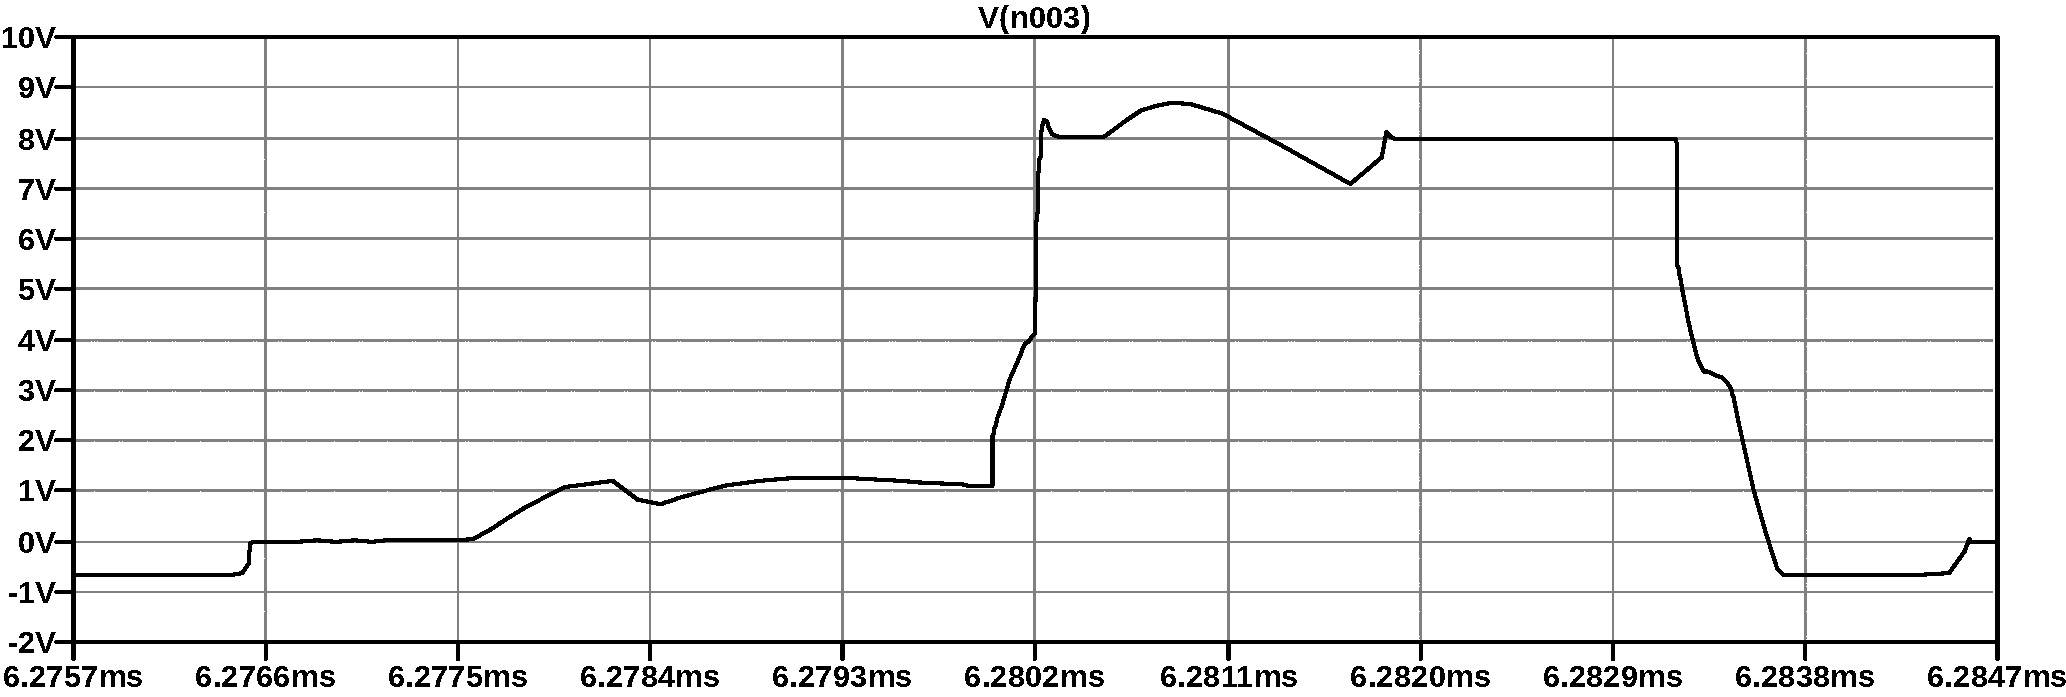
\includegraphics[width=\textwidth]{images/sim/1.pdf}
    \caption{Tensión de salida en el colector del TL494}
    \label{fig:sim:1}
\end{figure}

\begin{figure}[ht]
    \centering
    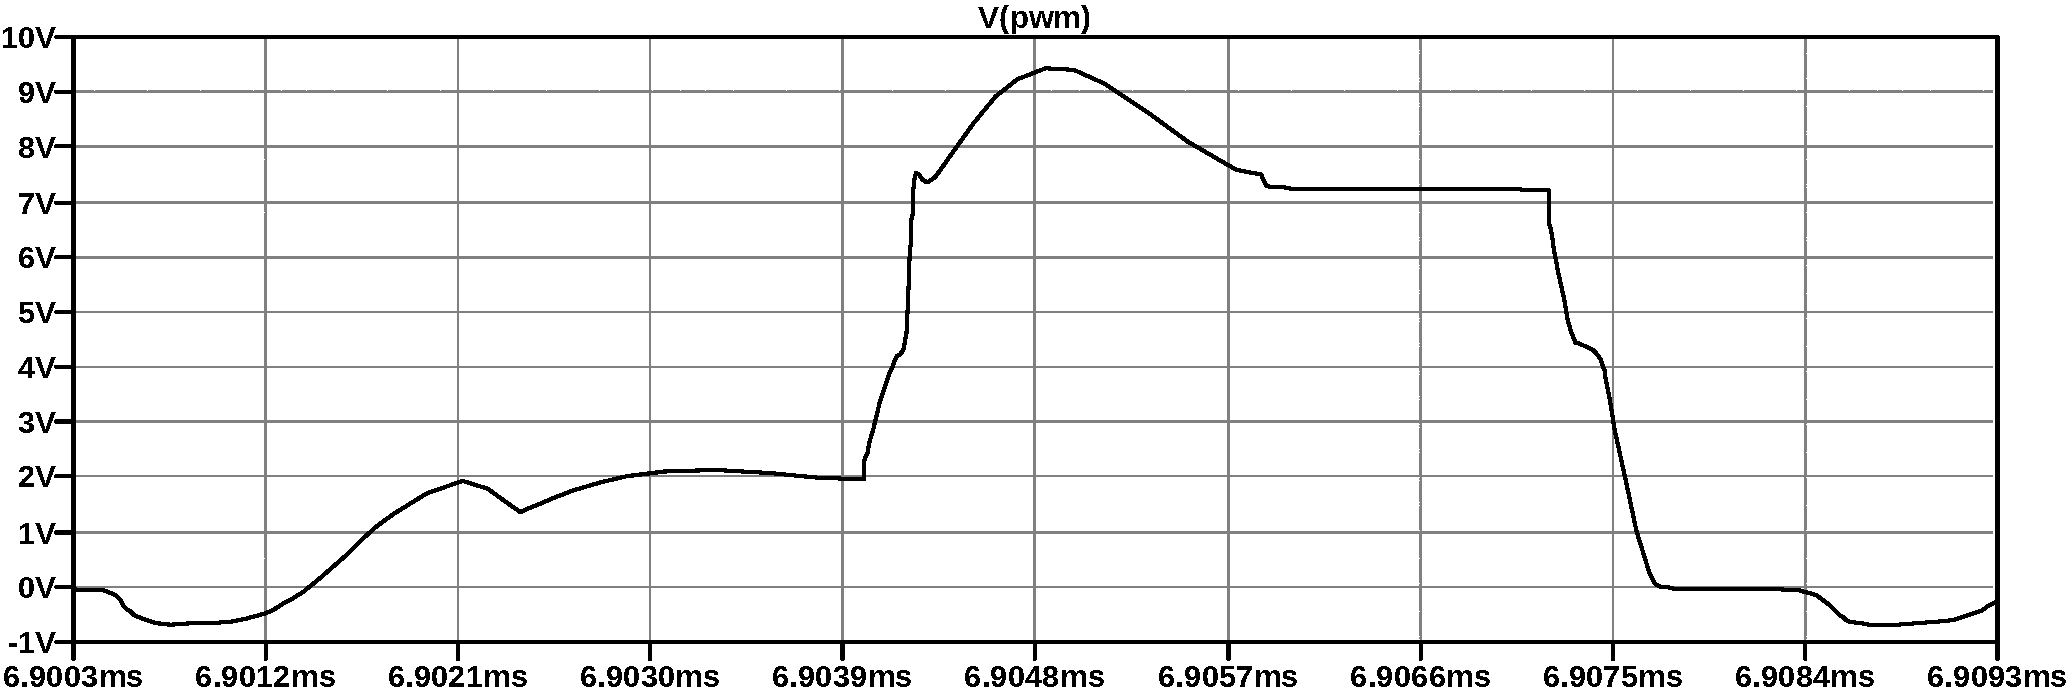
\includegraphics[width=\textwidth]{images/sim/3.pdf}
    \caption{Tensión de salida de la etapa de ganancia de corriente}
    \label{fig:sim:3}
\end{figure}

\begin{figure}[ht]
    \centering
    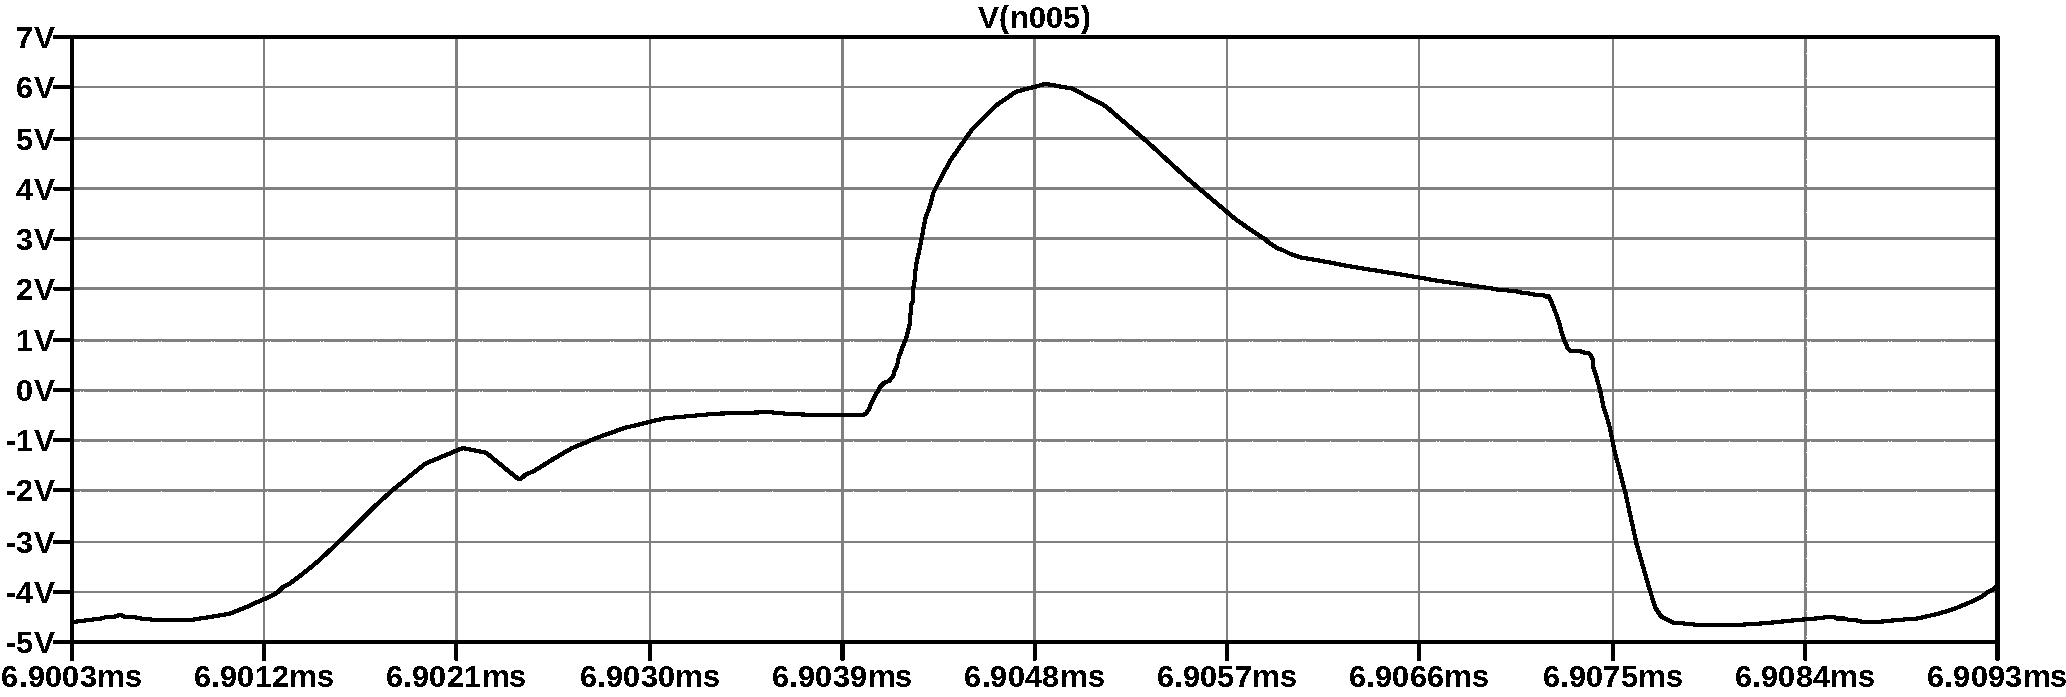
\includegraphics[width=\textwidth]{images/sim/4.pdf}
    \caption{Tensión en el primario del transformador del driver}
    \label{fig:sim:4}
\end{figure}

\begin{figure}[ht]
    \centering
    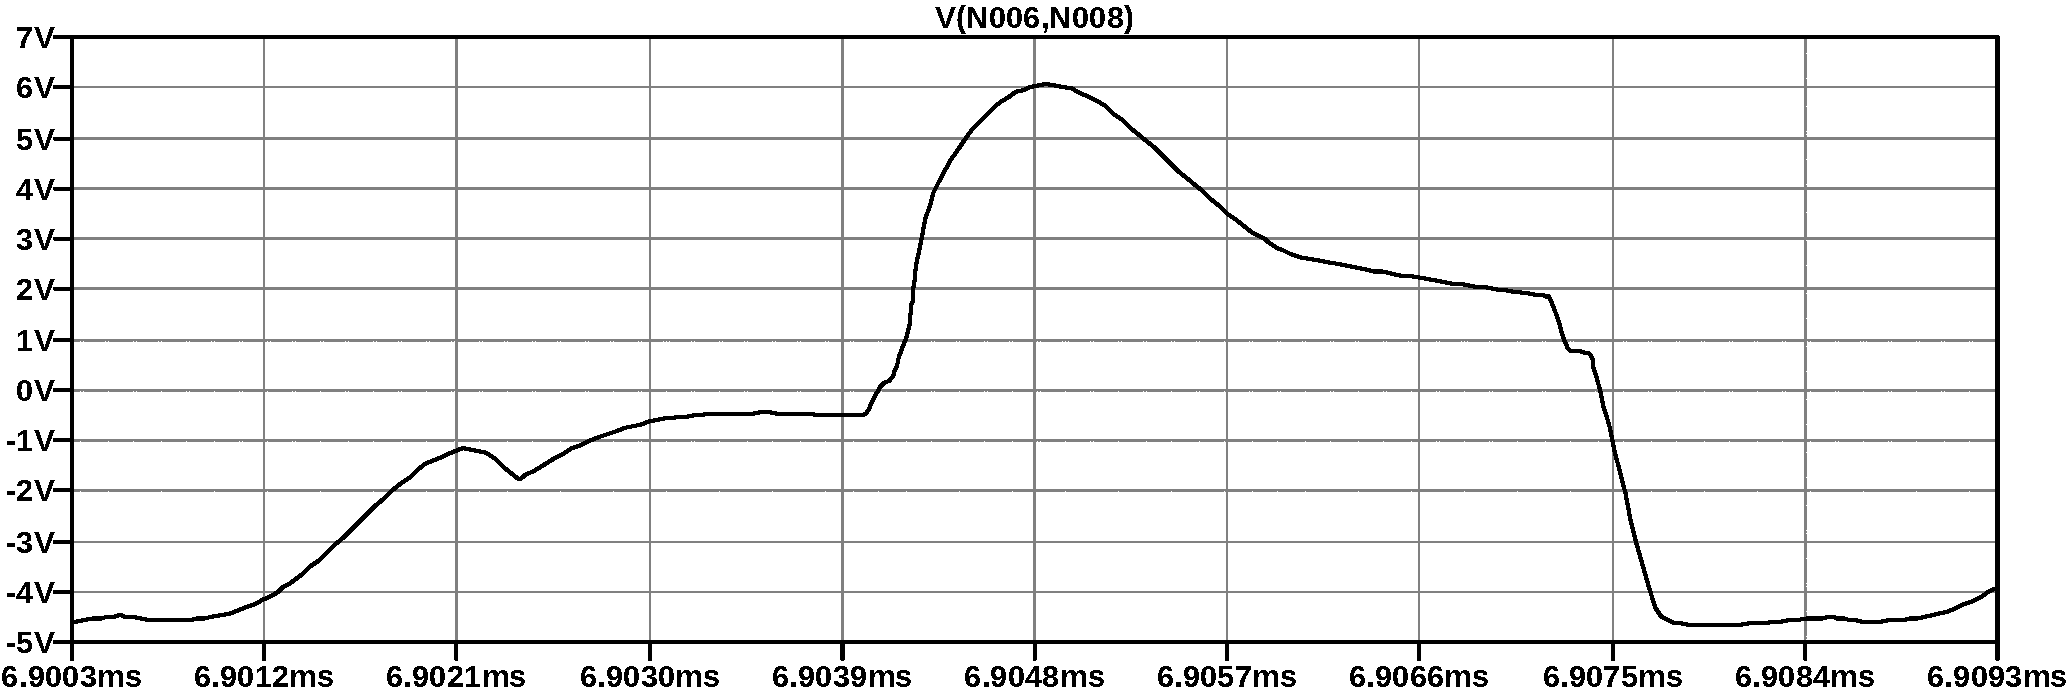
\includegraphics[width=\textwidth]{images/sim/5.pdf}
    \caption{Tensión en el secundario del transformador del driver}
    \label{fig:sim:5}
\end{figure}

\begin{figure}[ht]
    \centering
    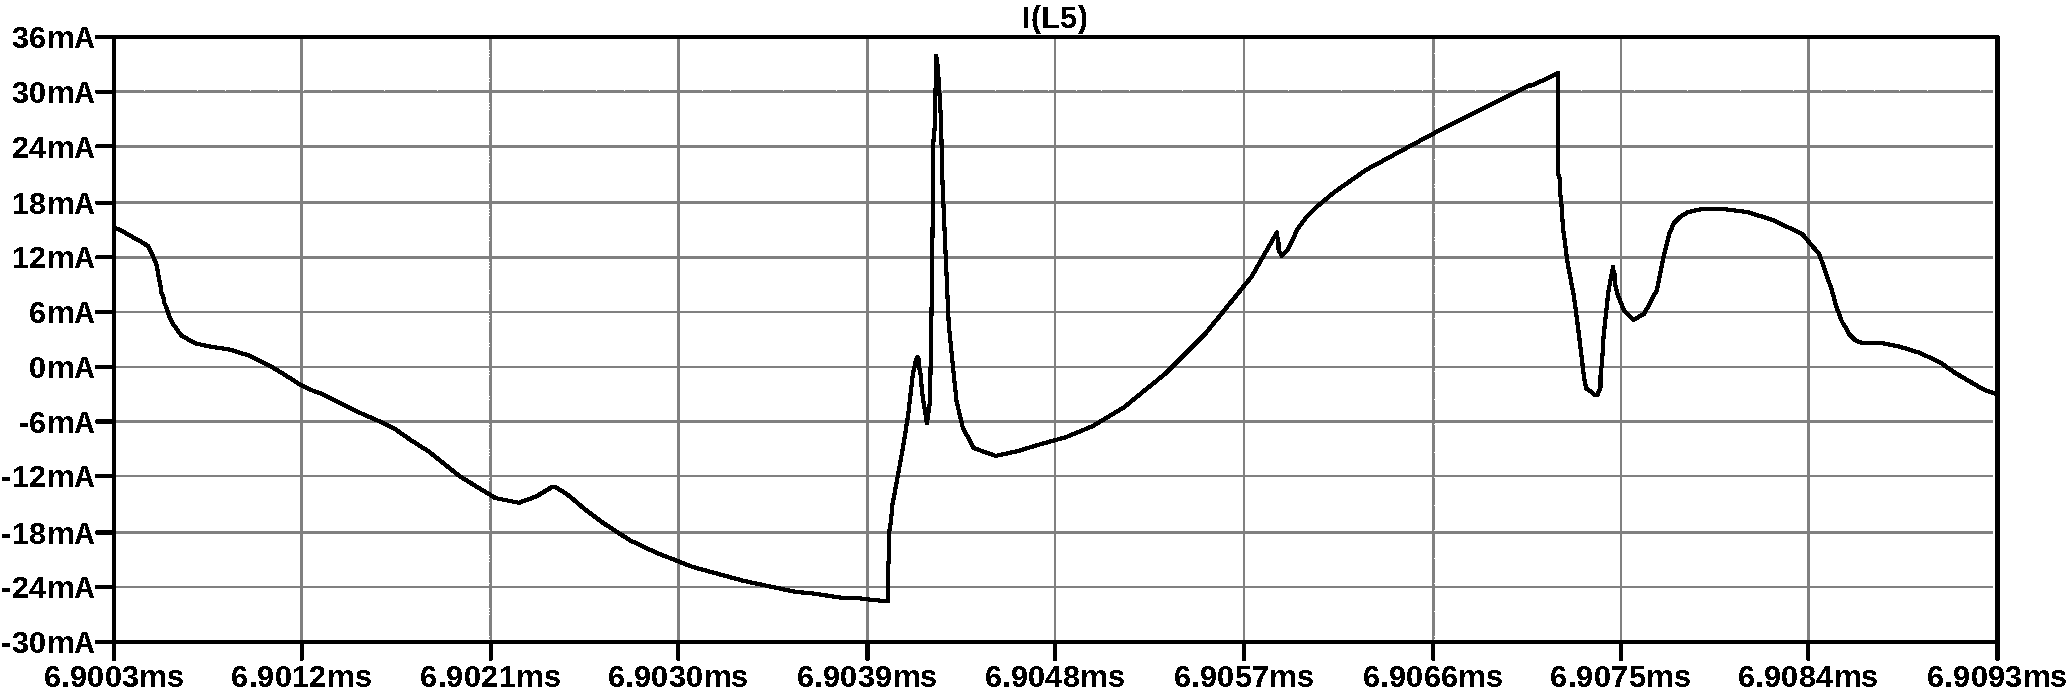
\includegraphics[width=\textwidth]{images/sim/6.pdf}
    \caption{Corriente en el primario del transformador del driver}
    \label{fig:sim:6}
\end{figure}

\begin{figure}[ht]
    \centering
    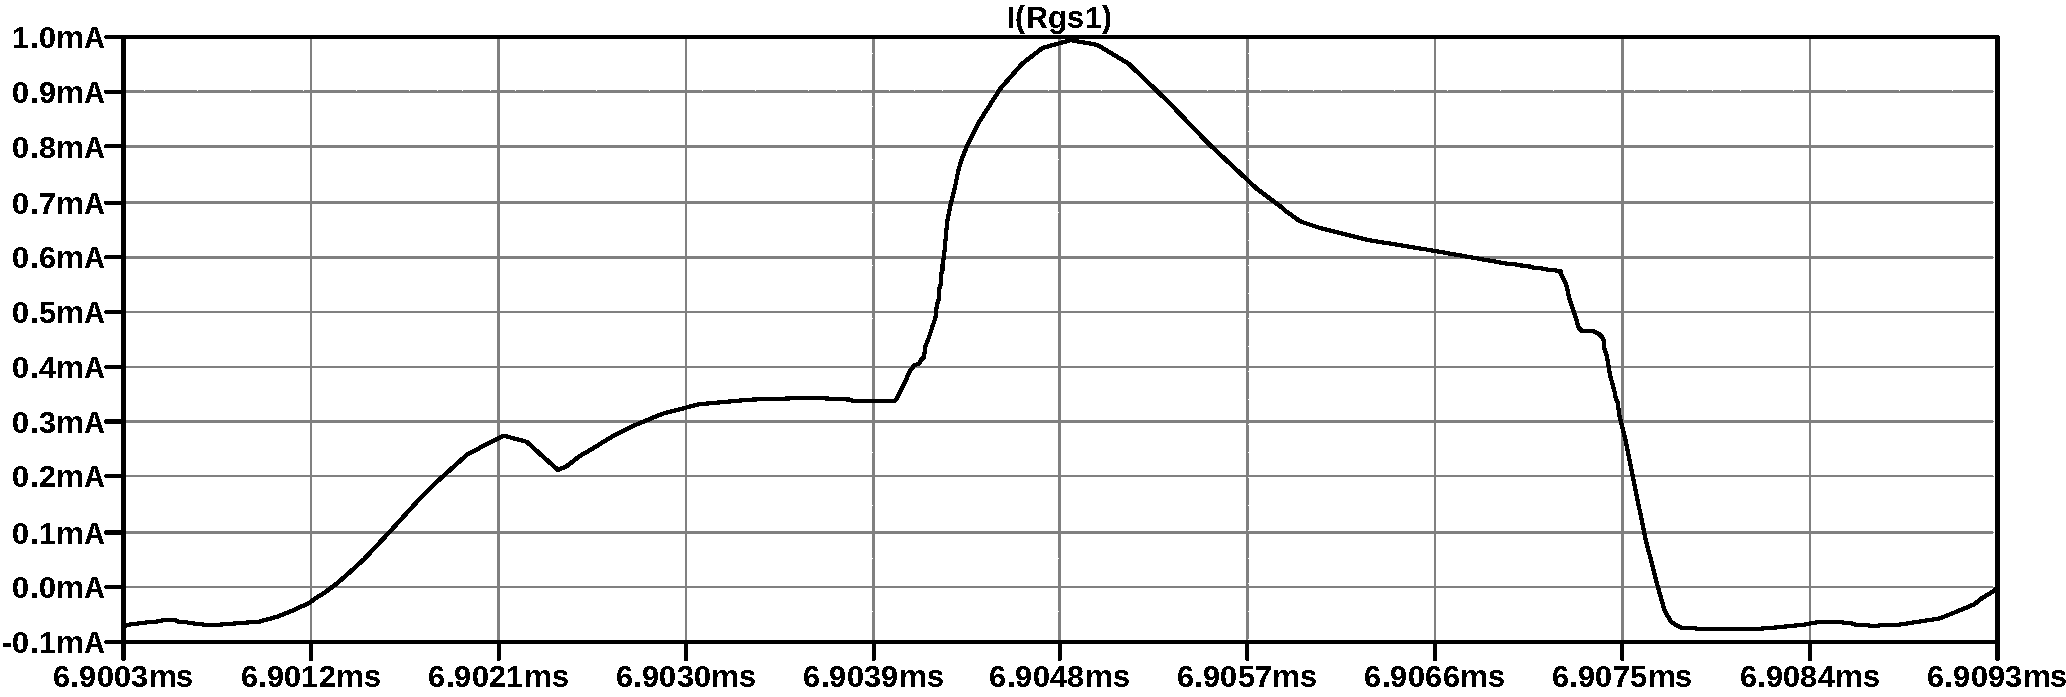
\includegraphics[width=\textwidth]{images/sim/7.pdf}
    \caption{Corriente en la resistencia entre gate y source del driver}
    \label{fig:sim:7}
\end{figure}

\begin{figure}[ht]
    \centering
    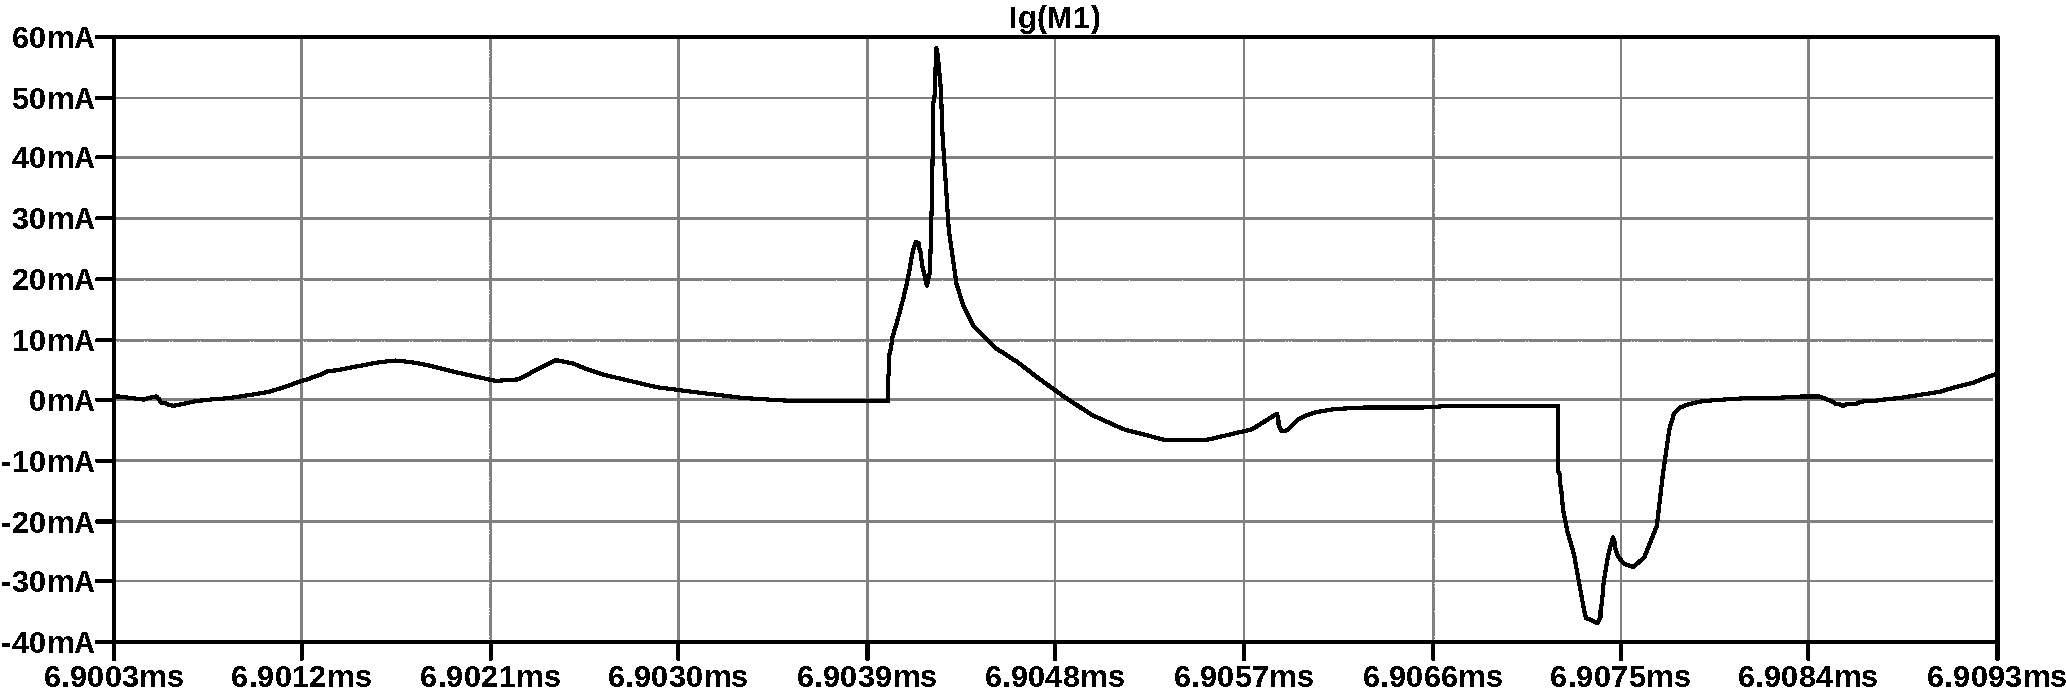
\includegraphics[width=\textwidth]{images/sim/8.pdf}
    \caption{Corriente que circula por el gate del MOSFET 1 (high side)}
    \label{fig:sim:8}
\end{figure}

\begin{figure}[ht]
    \centering
    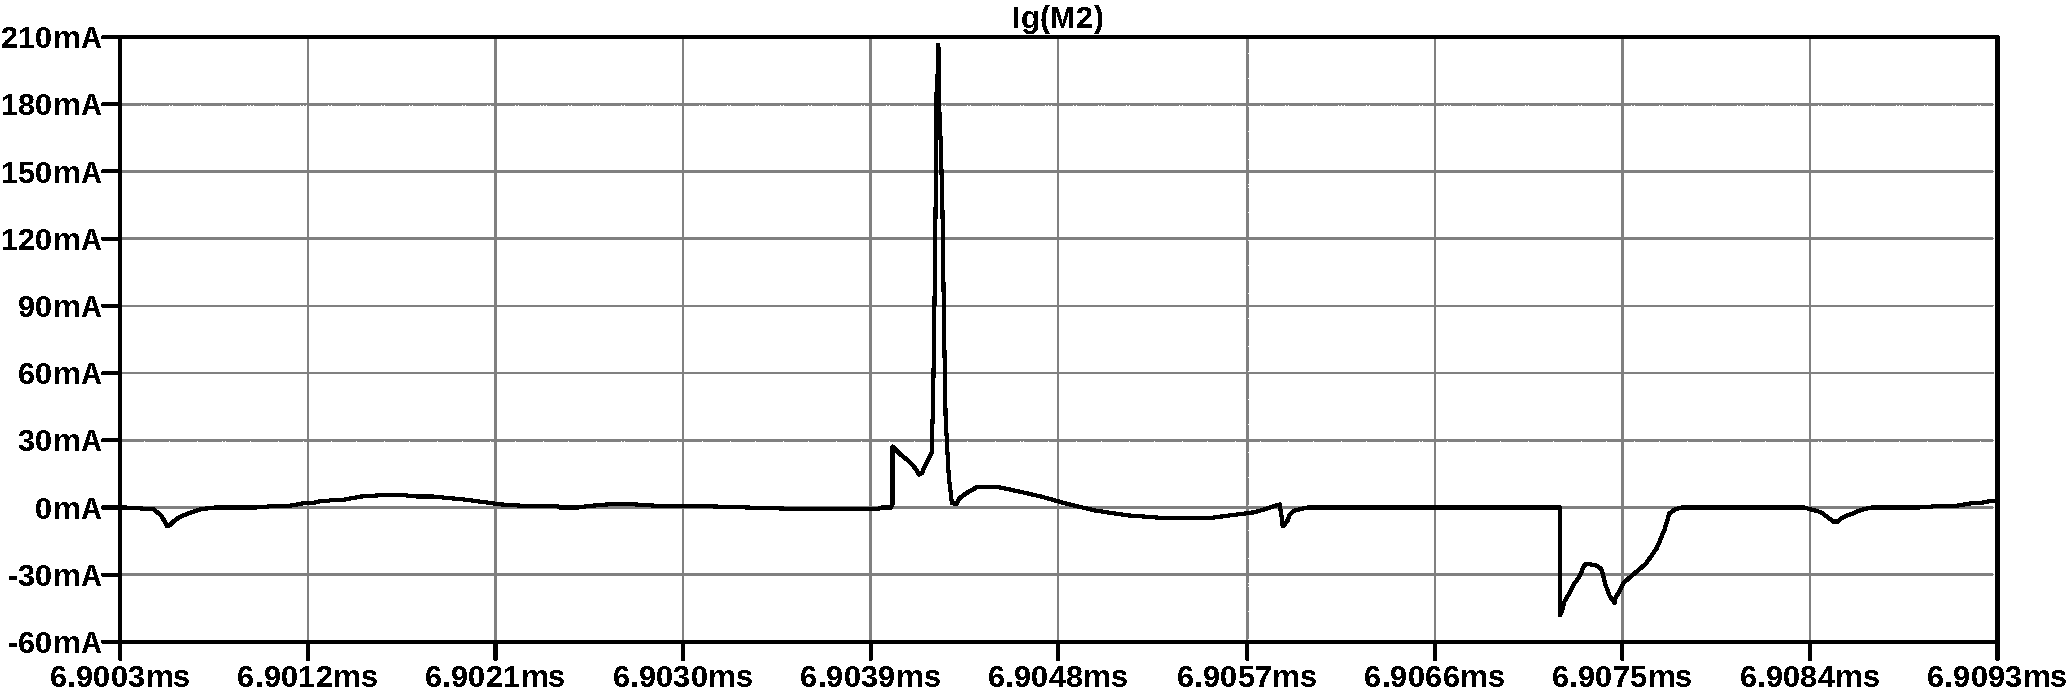
\includegraphics[width=\textwidth]{images/sim/9.pdf}
    \caption{Corriente que circula por el gate del MOSFET 2 (low side)}
    \label{fig:sim:9}
\end{figure}

\begin{figure}[ht]
    \centering
    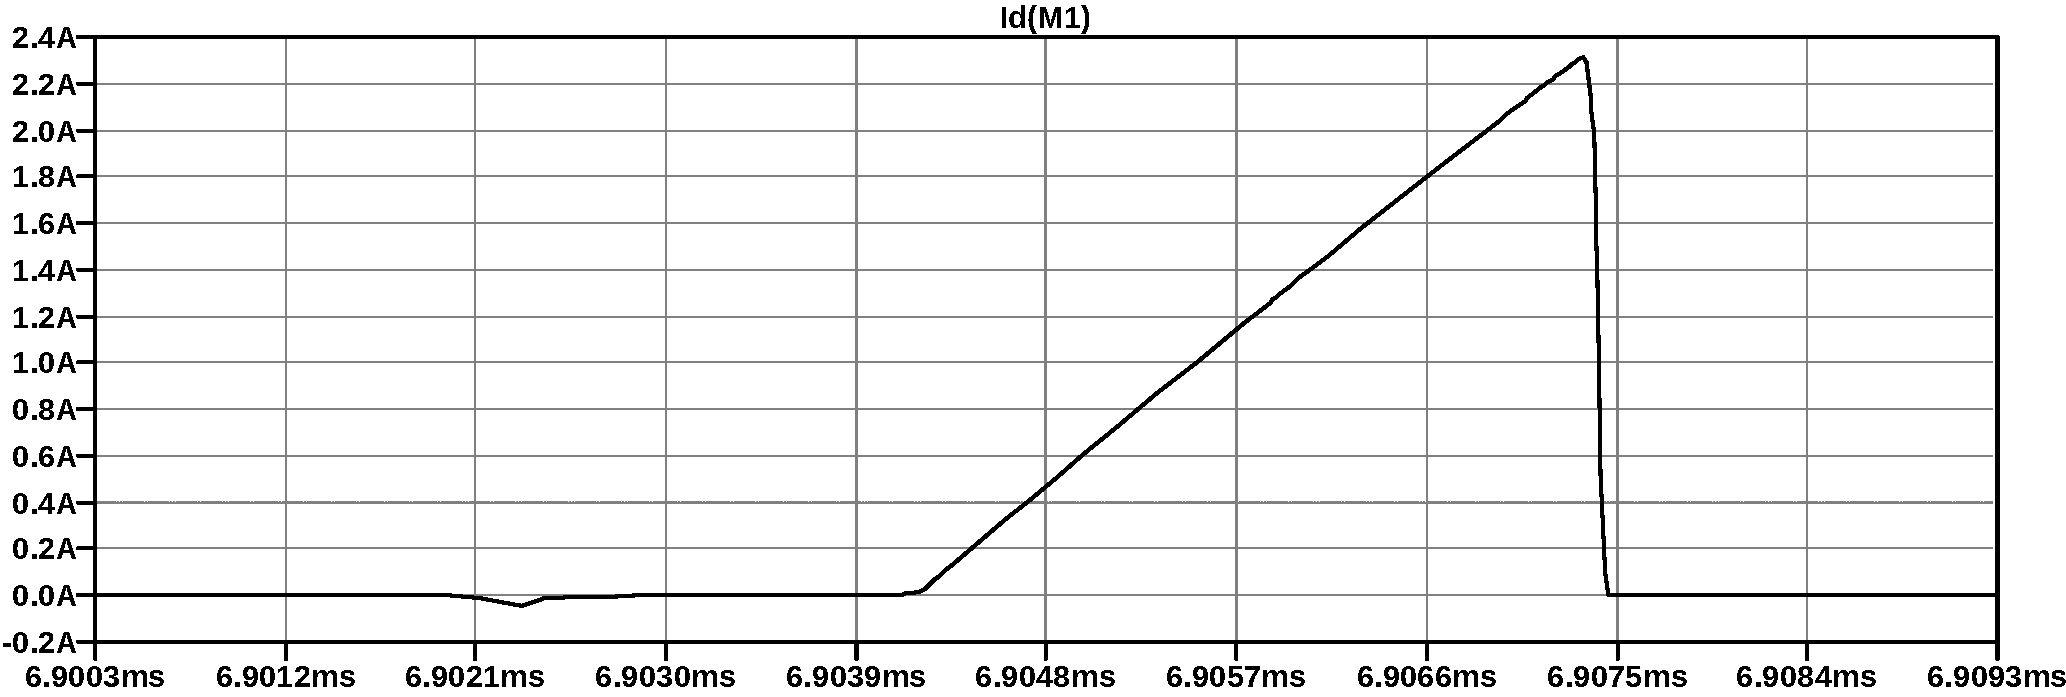
\includegraphics[width=\textwidth]{images/sim/10.pdf}
    \caption{Corriente que circula por el drain del MOSFET 1 (high side)}
    \label{fig:sim:10}
\end{figure}

\begin{figure}[ht]
    \centering
    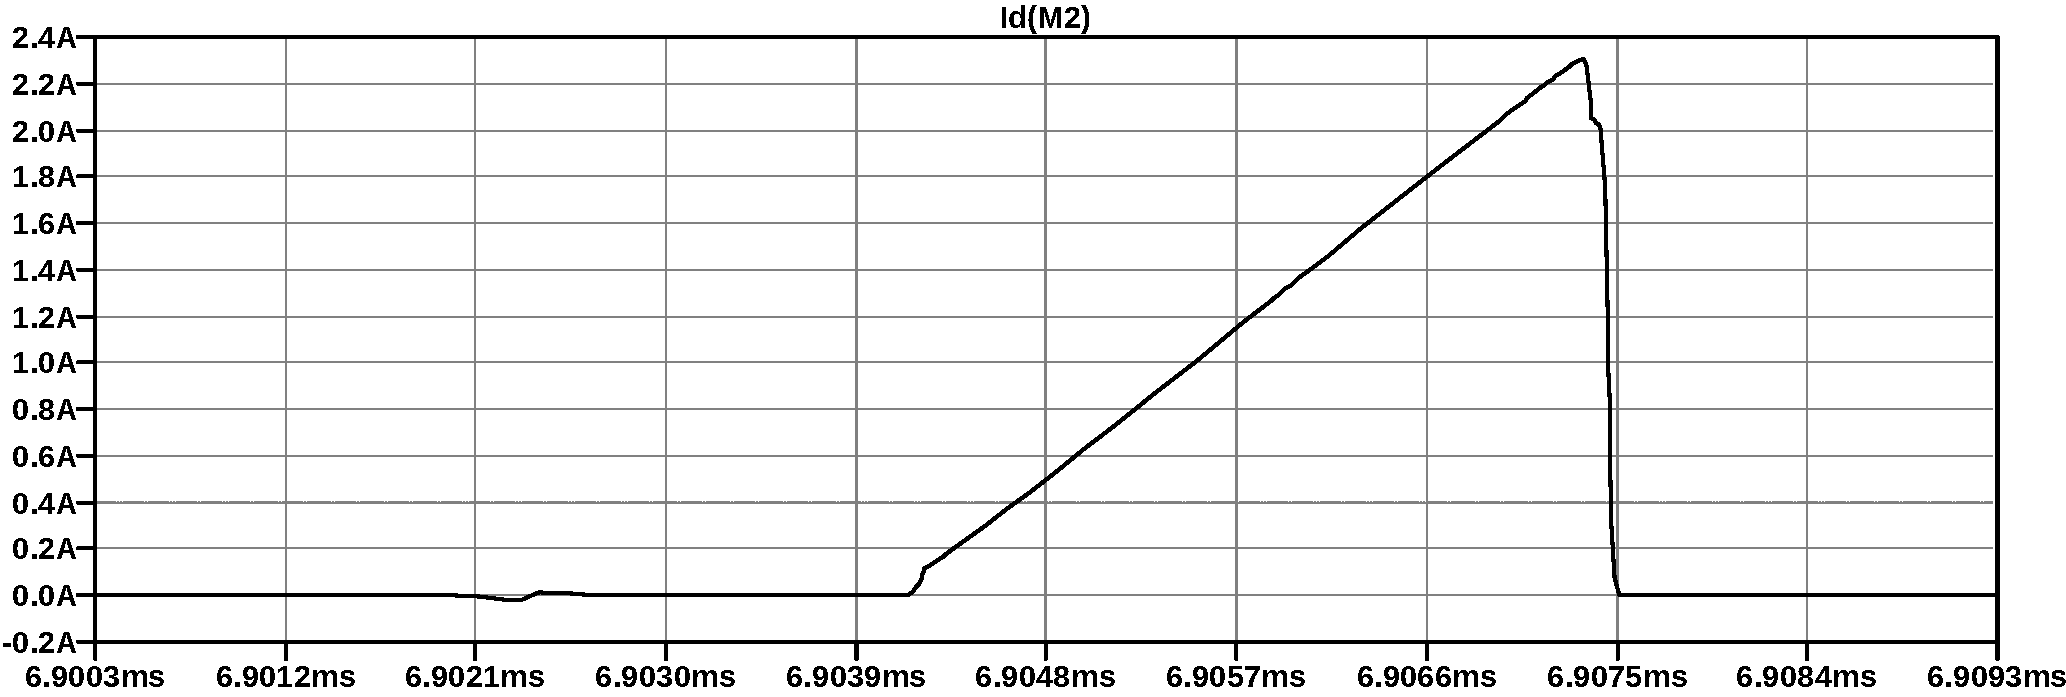
\includegraphics[width=\textwidth]{images/sim/11.pdf}
    \caption{Corriente que circula por el drain del MOSFET 2 (low side)}
    \label{fig:sim:11}
\end{figure}

\begin{figure}[ht]
    \centering
    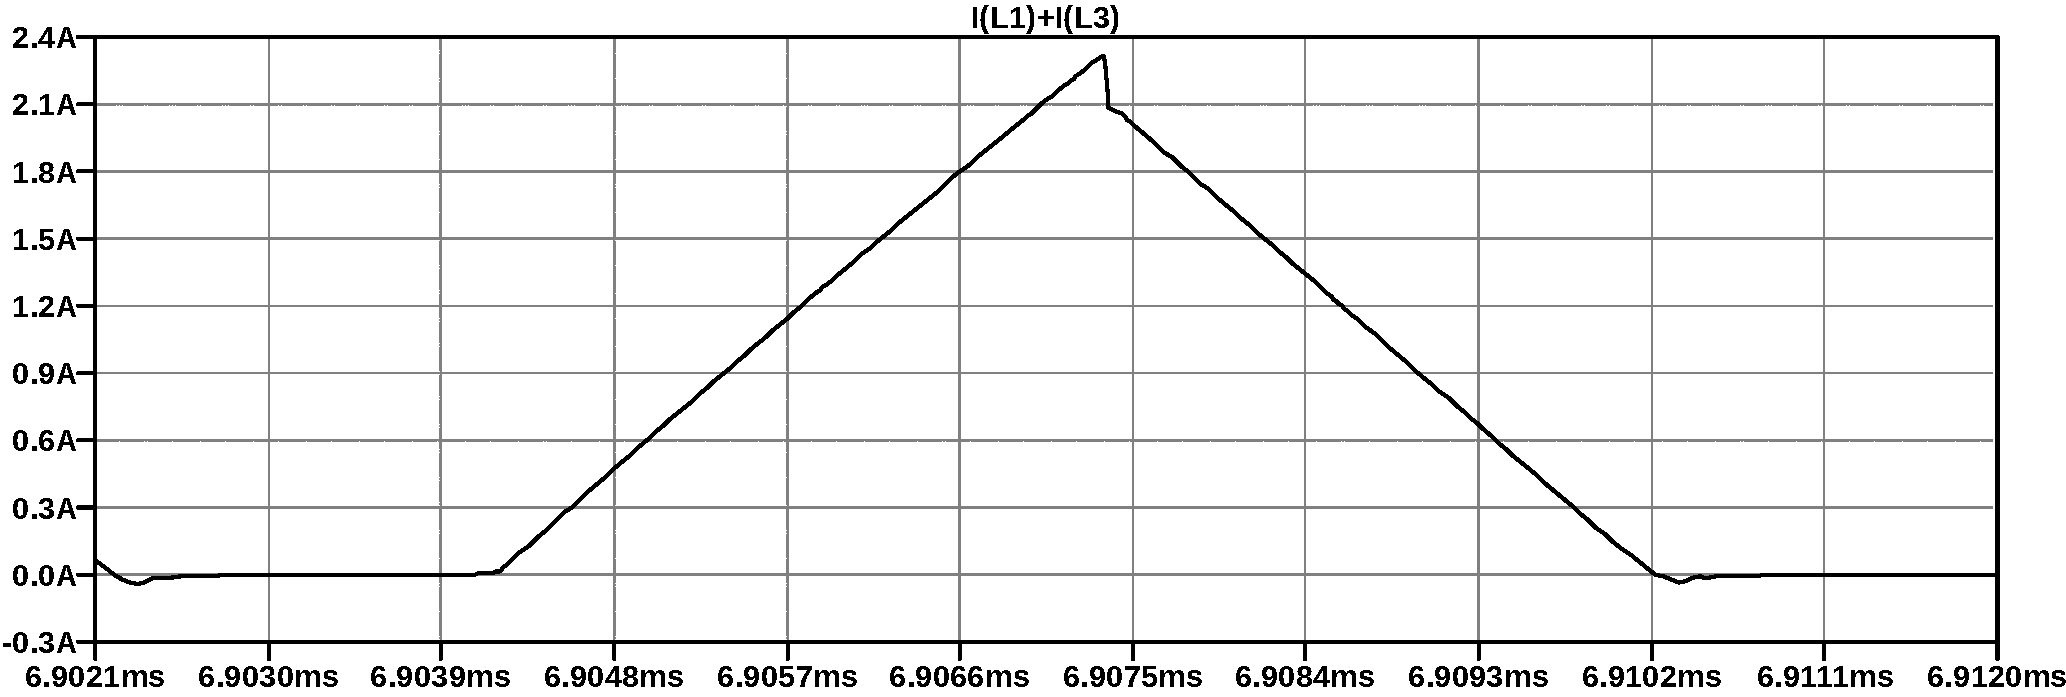
\includegraphics[width=\textwidth]{images/sim/12.pdf}
    \caption{Corriente en el primario del transformador de potencia}
    \label{fig:sim:12}
\end{figure}

\begin{figure}[ht]
    \centering
    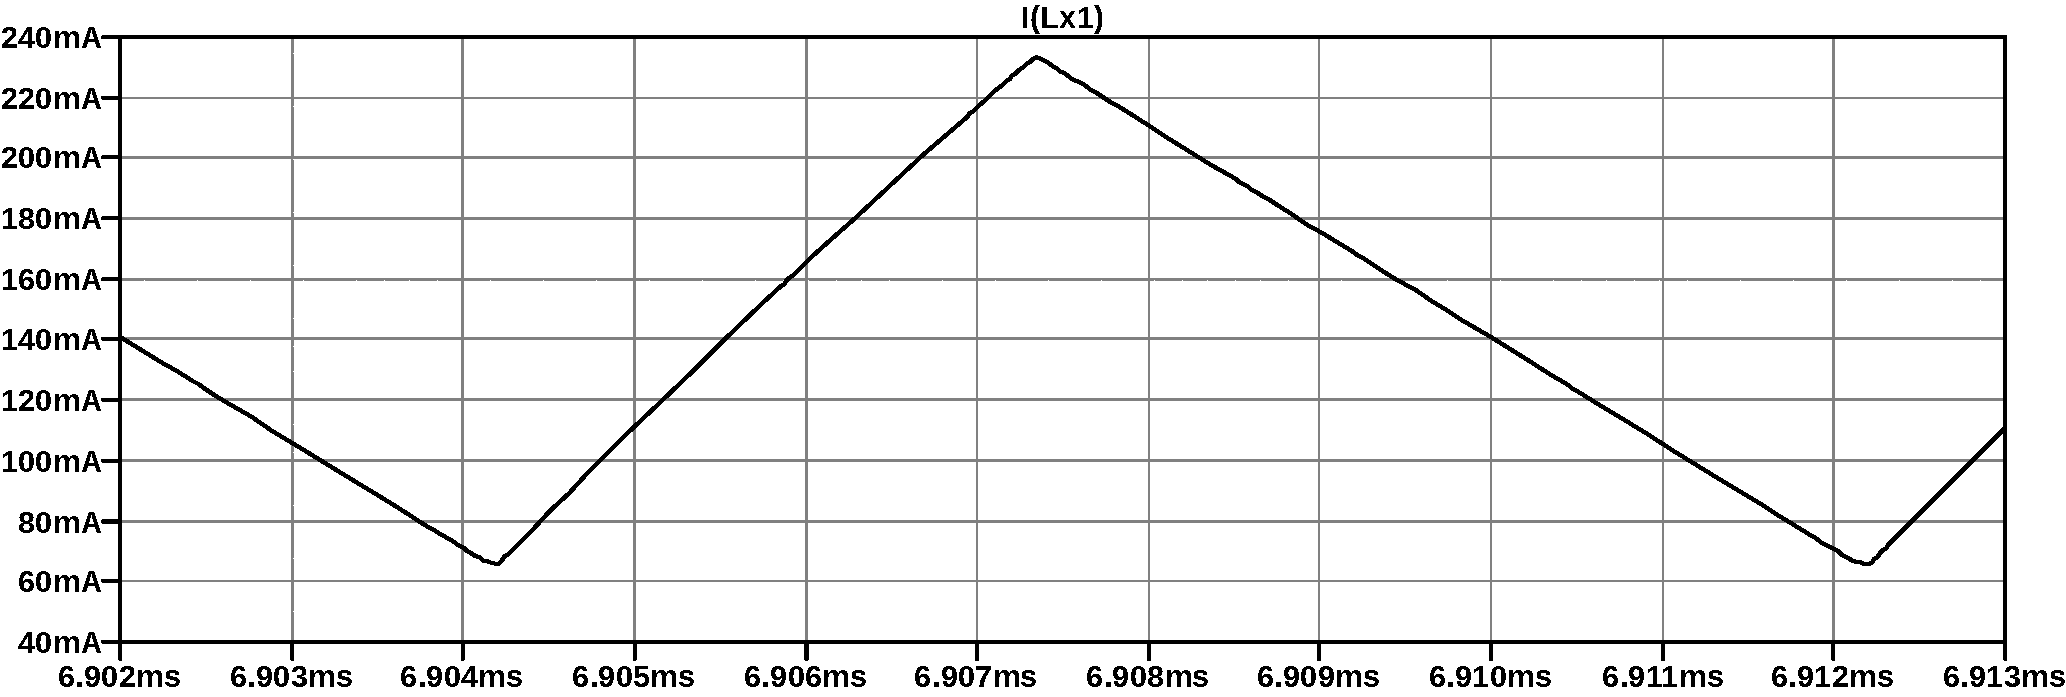
\includegraphics[width=\textwidth]{images/sim/13.pdf}
    \caption{Corriente en el inductor del filtro de salida}
    \label{fig:sim:13}
\end{figure}

\begin{figure}[ht]
    \centering
    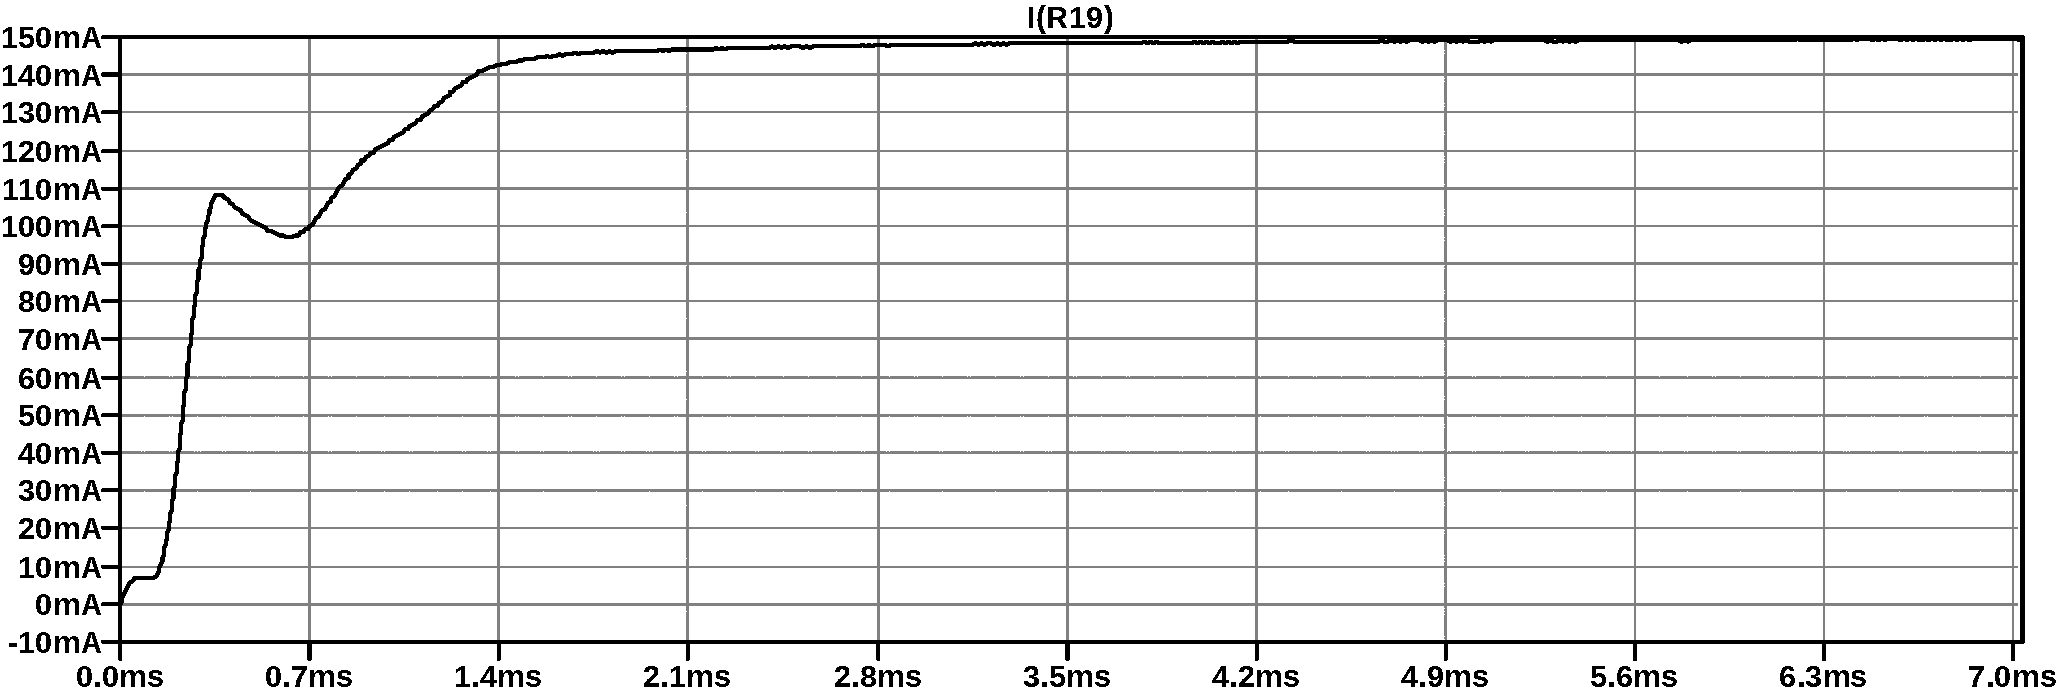
\includegraphics[width=\textwidth]{images/sim/14.pdf}
    \caption{Corriente por la carga y su ripple}
    \label{fig:sim:14}
\end{figure}

\begin{figure}[ht]
    \centering
    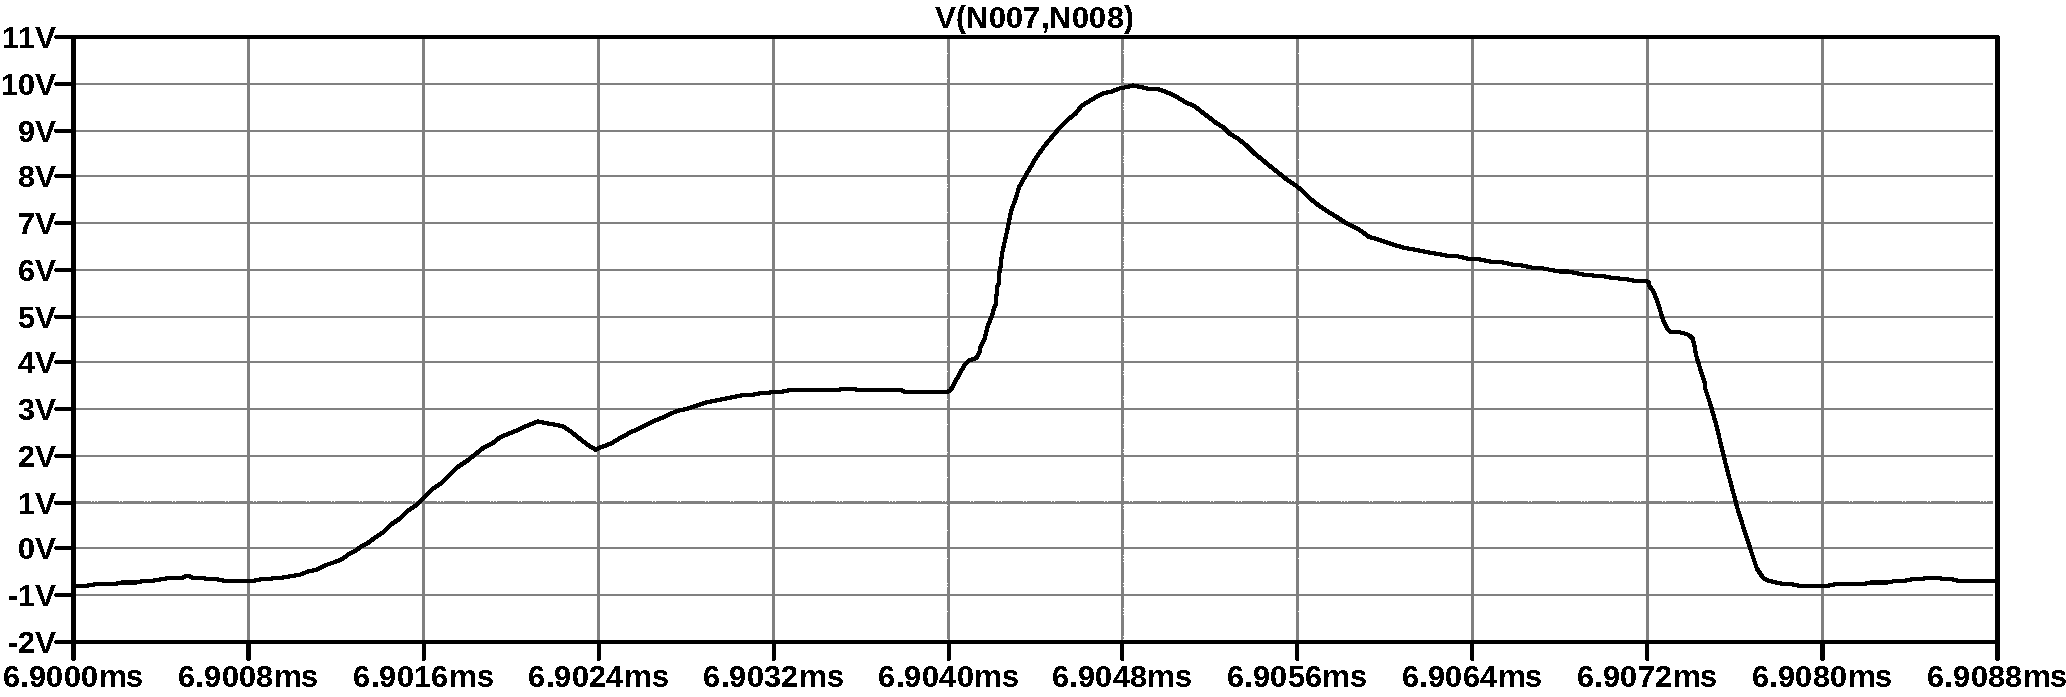
\includegraphics[width=\textwidth]{images/sim/15.pdf}
    \caption{Tensión entre gate y source del MOSFET 1 (high side)}
    \label{fig:sim:15}
\end{figure}

\begin{figure}[ht]
    \centering
    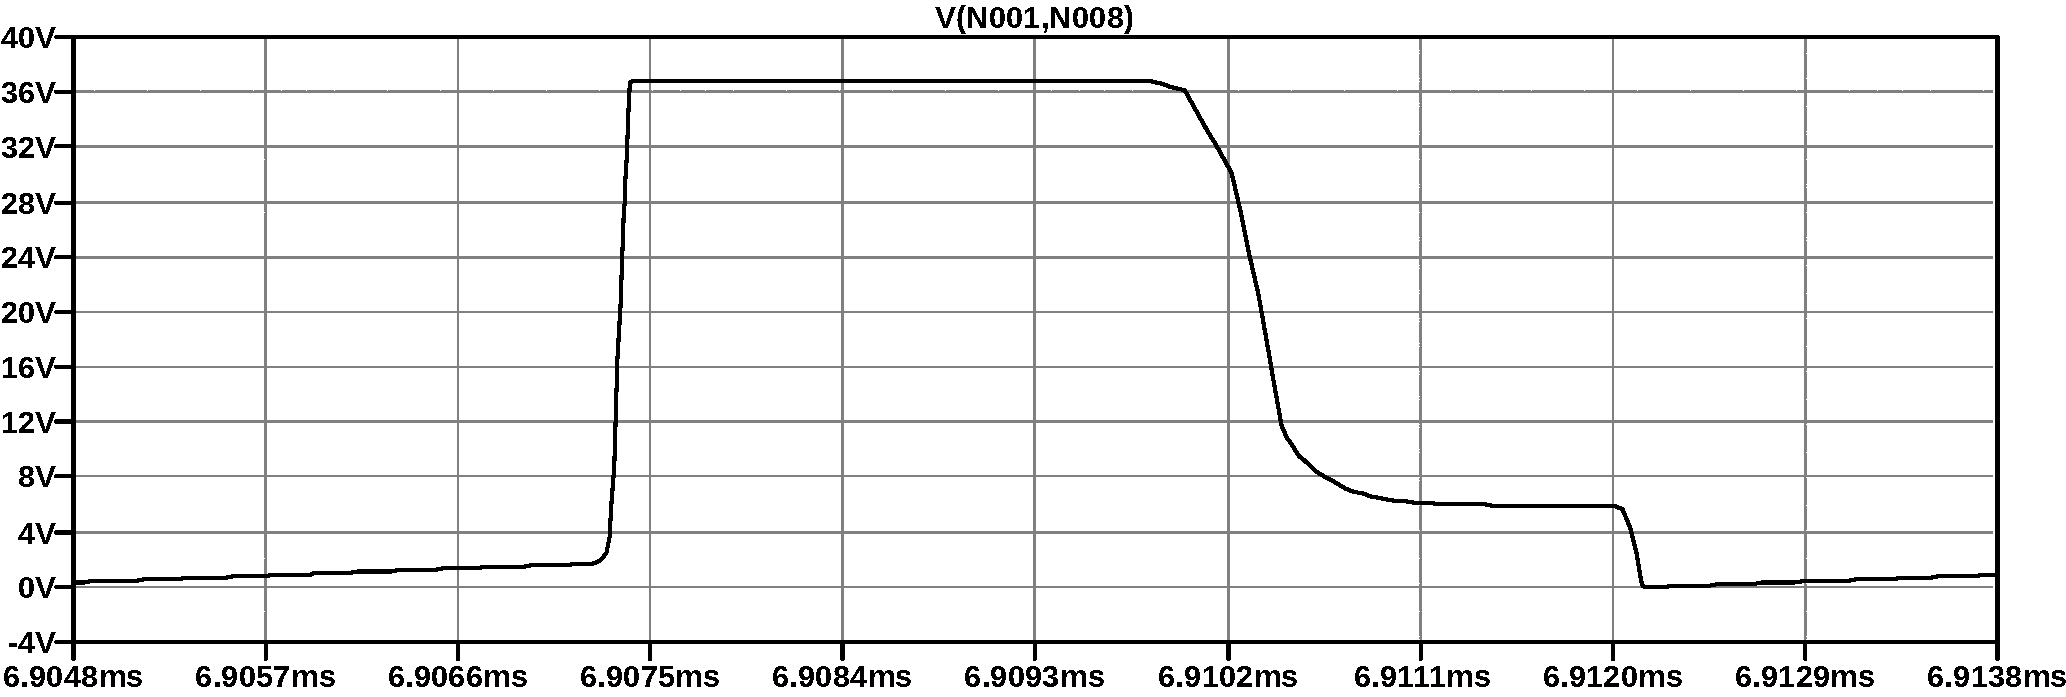
\includegraphics[width=\textwidth]{images/sim/16.pdf}
    \caption{Tensión entre drain y source del MOSFET 1 (high side)}
    \label{fig:sim:16}
\end{figure}

\begin{figure}[ht]
    \centering
    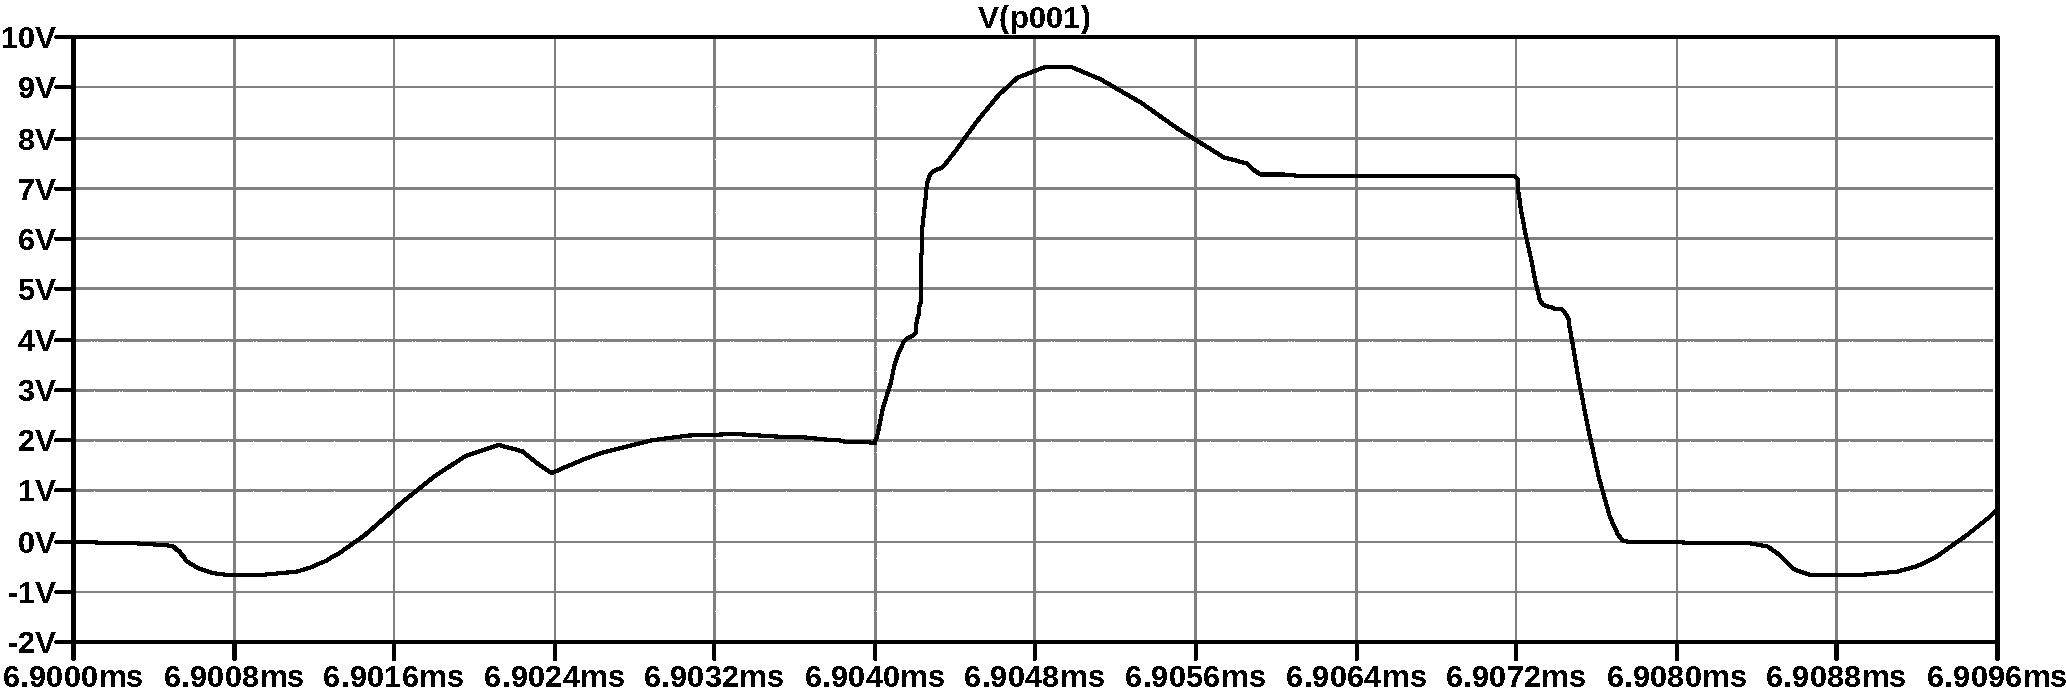
\includegraphics[width=\textwidth]{images/sim/17.pdf}
    \caption{Tensión entre gate y source del MOSFET 2 (low side)}
    \label{fig:sim:17}
\end{figure}

\begin{figure}[ht]
    \centering
    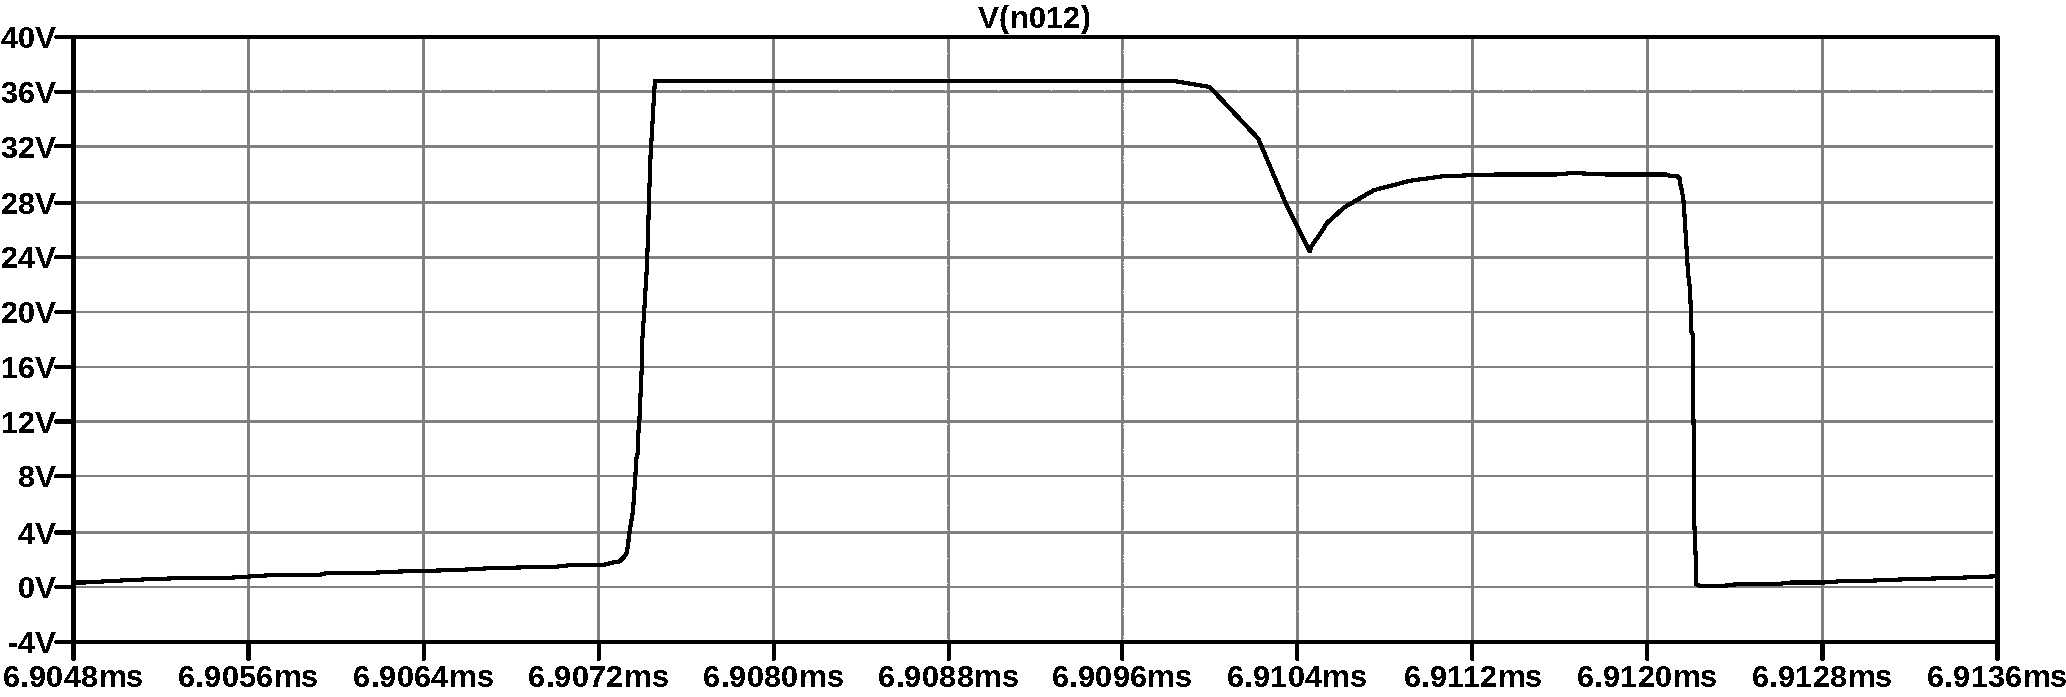
\includegraphics[width=\textwidth]{images/sim/18.pdf}
    \caption{Tensión entre drain y source del MOSFET 2 (low side)}
    \label{fig:sim:18}
\end{figure}

\begin{figure}[ht]
    \centering
    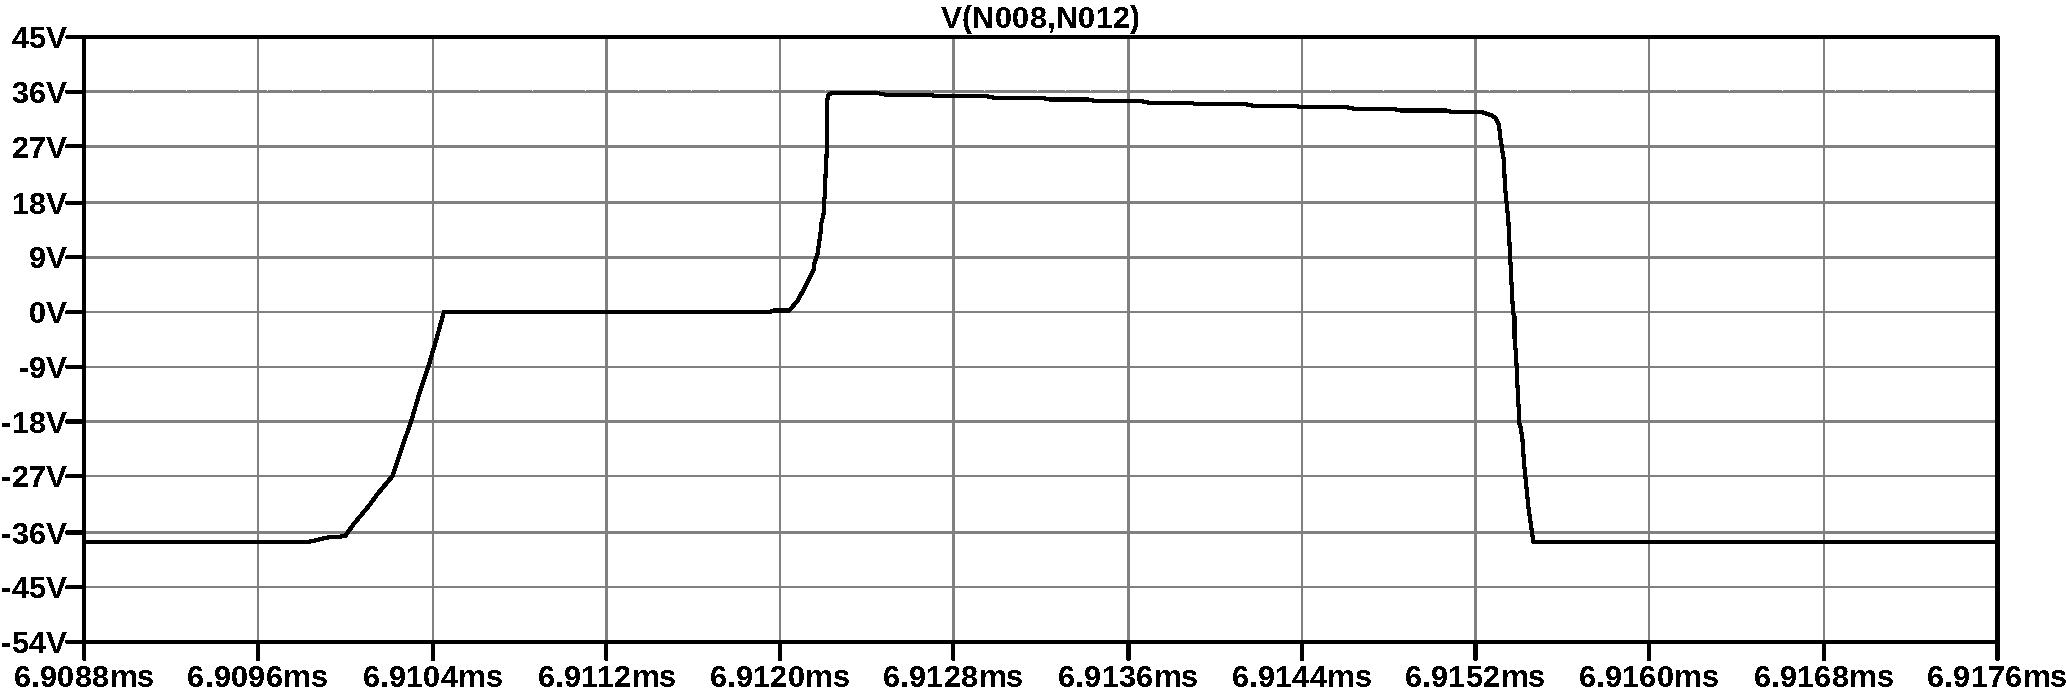
\includegraphics[width=\textwidth]{images/sim/19.pdf}
    \caption{Tensión en el primario del transformador de potencia}
    \label{fig:sim:19}
\end{figure}

\begin{figure}[ht]
    \centering
    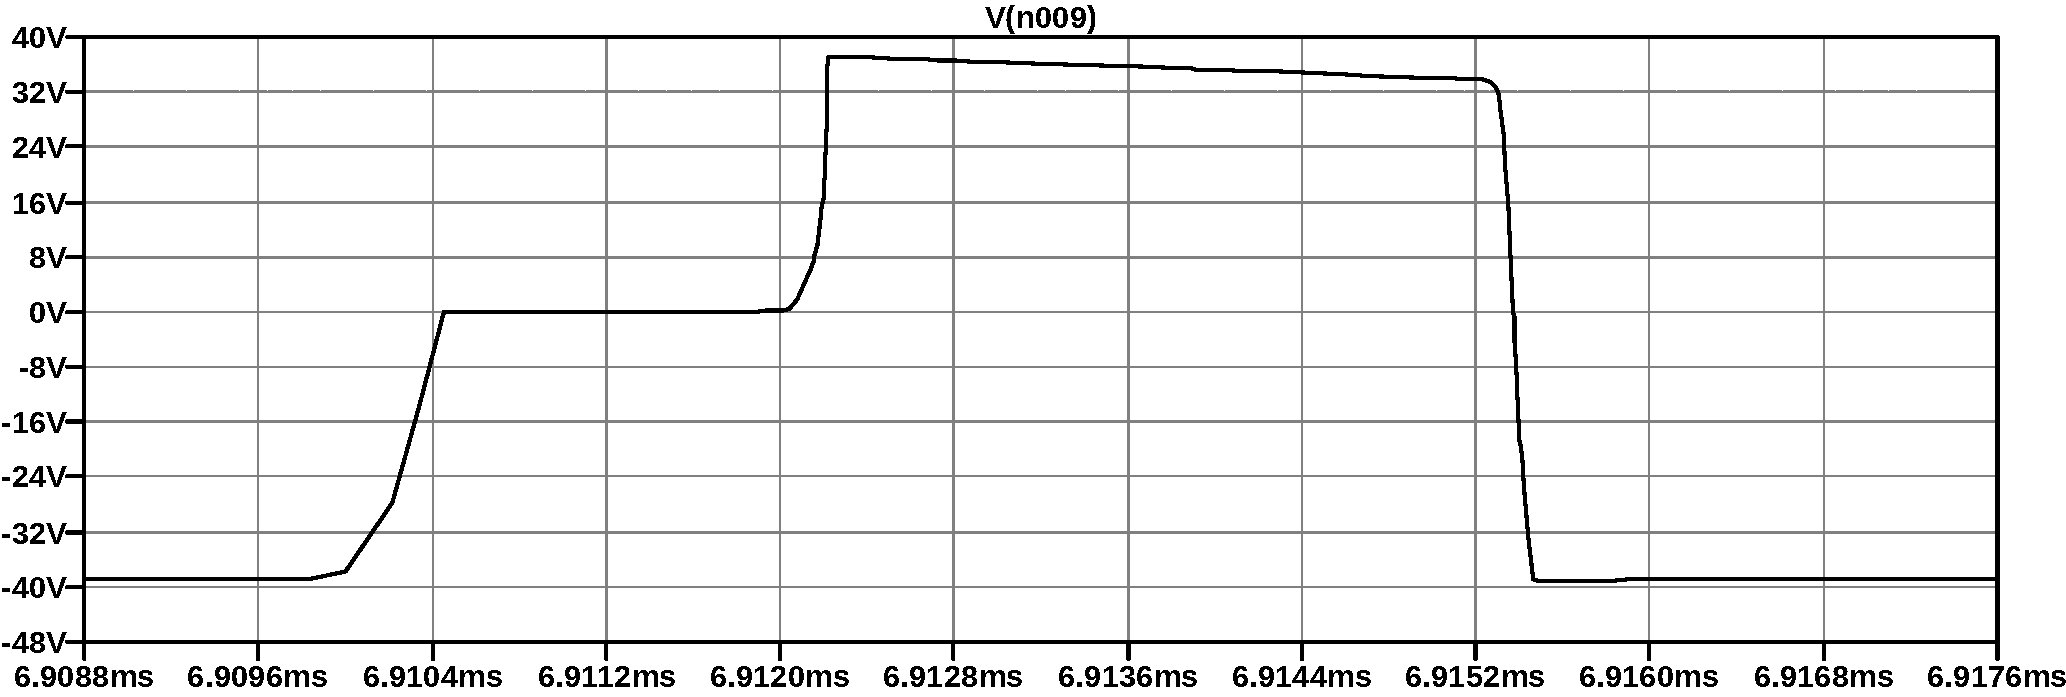
\includegraphics[width=\textwidth]{images/sim/20.pdf}
    \caption{Tensión en el secundario del transformador de potencia}
    \label{fig:sim:20}
\end{figure}

\begin{figure}[ht]
    \centering
    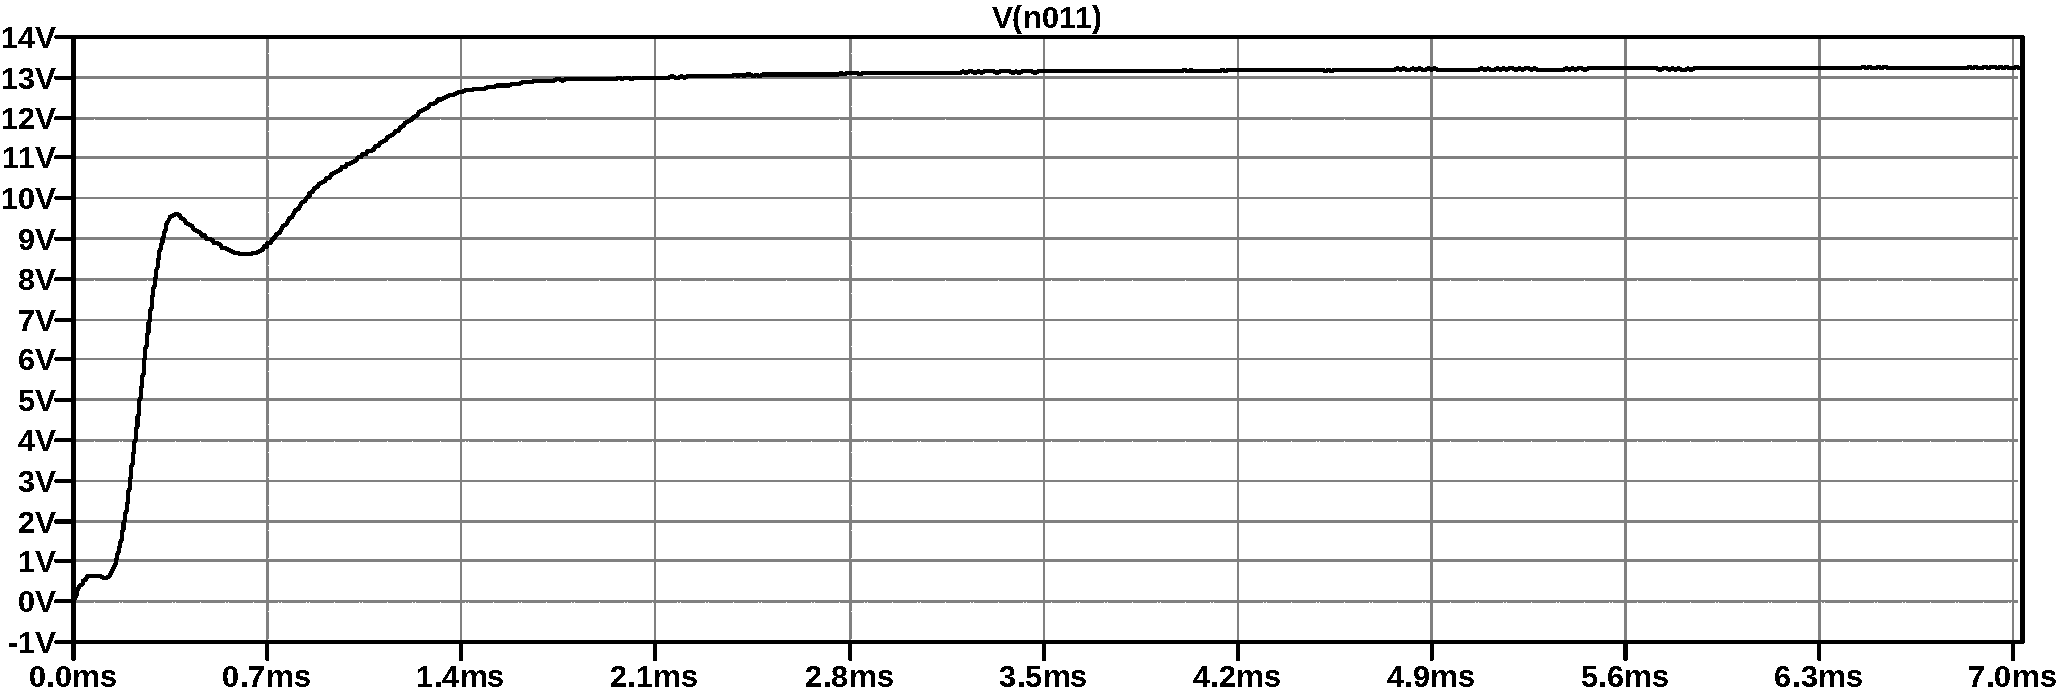
\includegraphics[width=\textwidth]{images/sim/21.pdf}
    \caption{Tensión en la carga y su ripple}
    \label{fig:sim:21}
\end{figure}

\begin{figure}[ht]
    \centering
    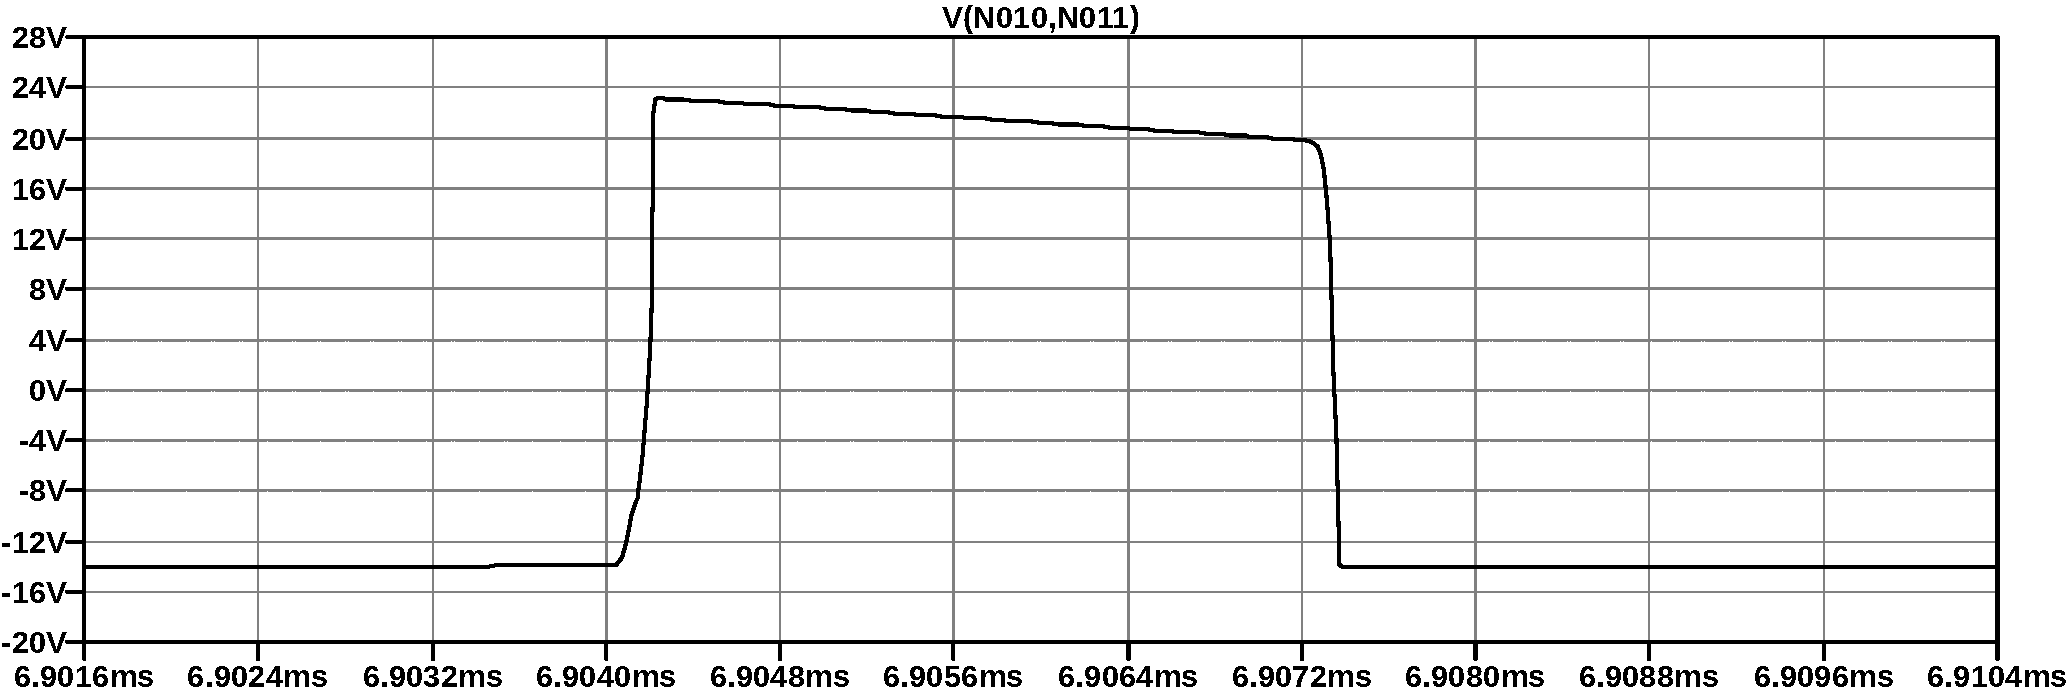
\includegraphics[width=\textwidth]{images/sim/22.pdf}
    \caption{Tensión en el inductor del filtro de salida}
    \label{fig:sim:22}
\end{figure}

\begin{figure}[ht]
    \centering
    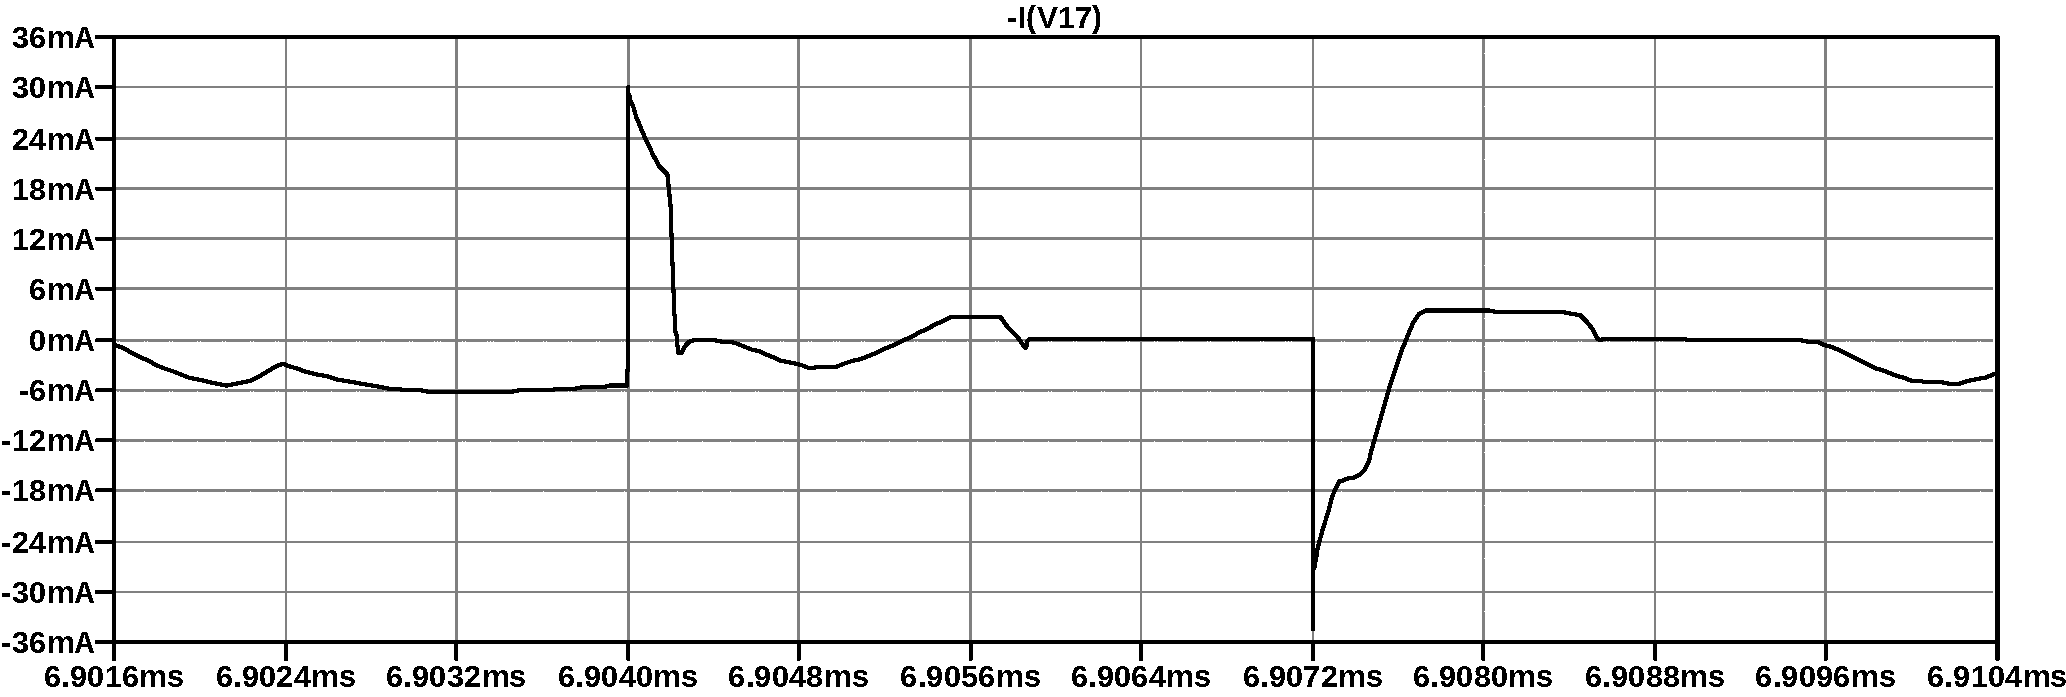
\includegraphics[width=\textwidth]{images/sim/23.pdf}
    \caption{Corriente de salida por colector del TL494}
    \label{fig:sim:23}
\end{figure}

\begin{figure}[ht]
    \centering
    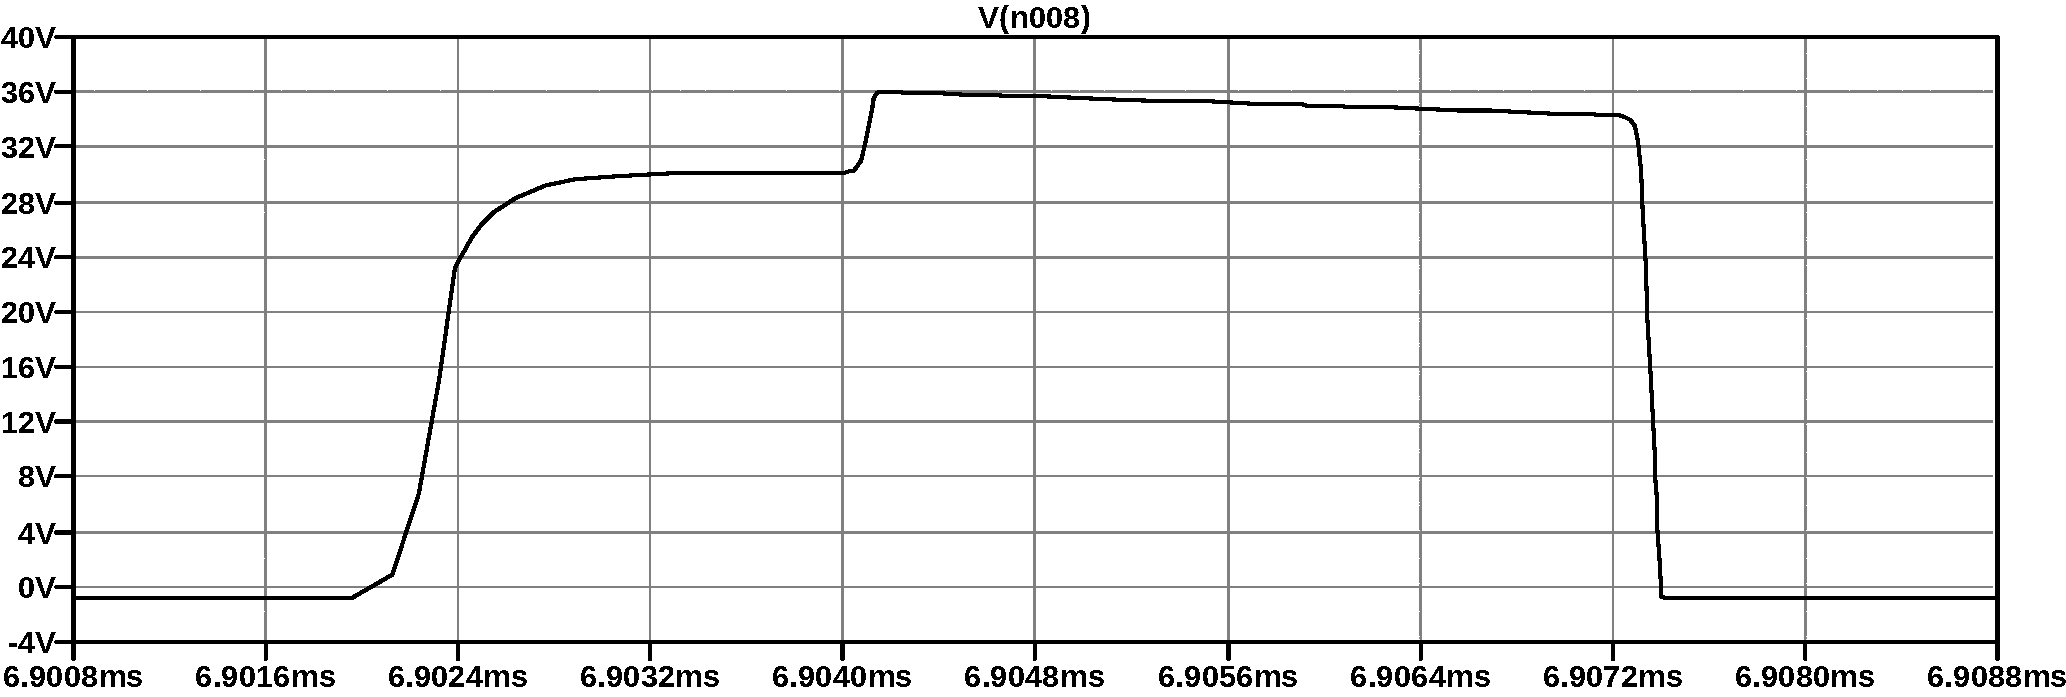
\includegraphics[width=\textwidth]{images/sim/24.pdf}
    \caption{Tensión cátodo ánodo en el diodo D1}
    \label{fig:sim:24}
\end{figure}

\begin{figure}[ht]
    \centering
    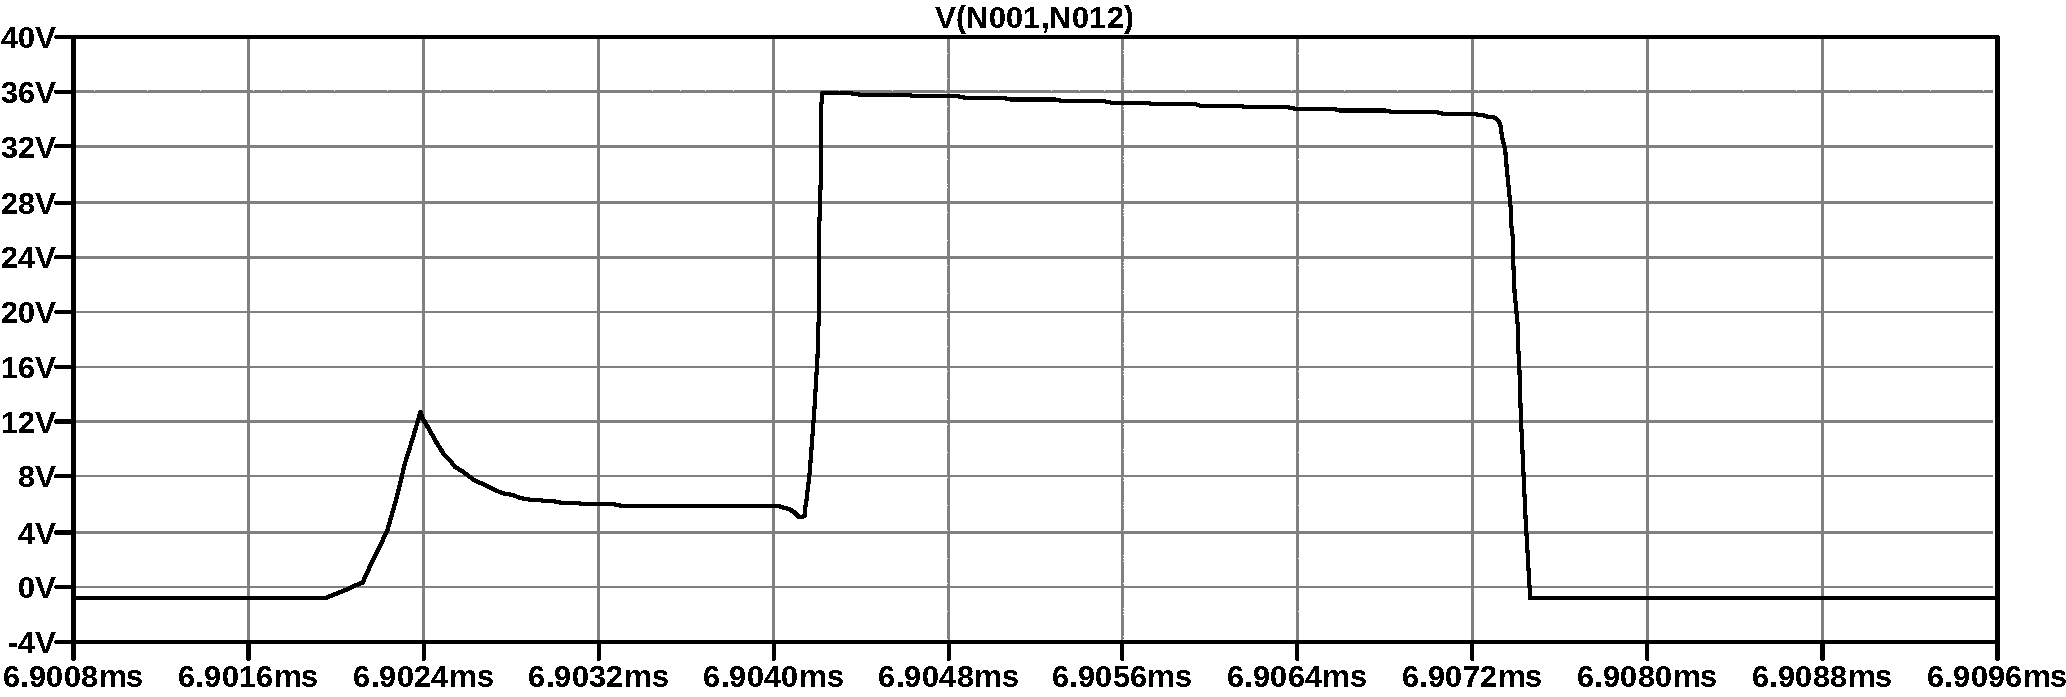
\includegraphics[width=\textwidth]{images/sim/25.pdf}
    \caption{Tensión cátodo ánodo en el diodo D2}
    \label{fig:sim:25}
\end{figure}

\begin{figure}[ht]
    \centering
    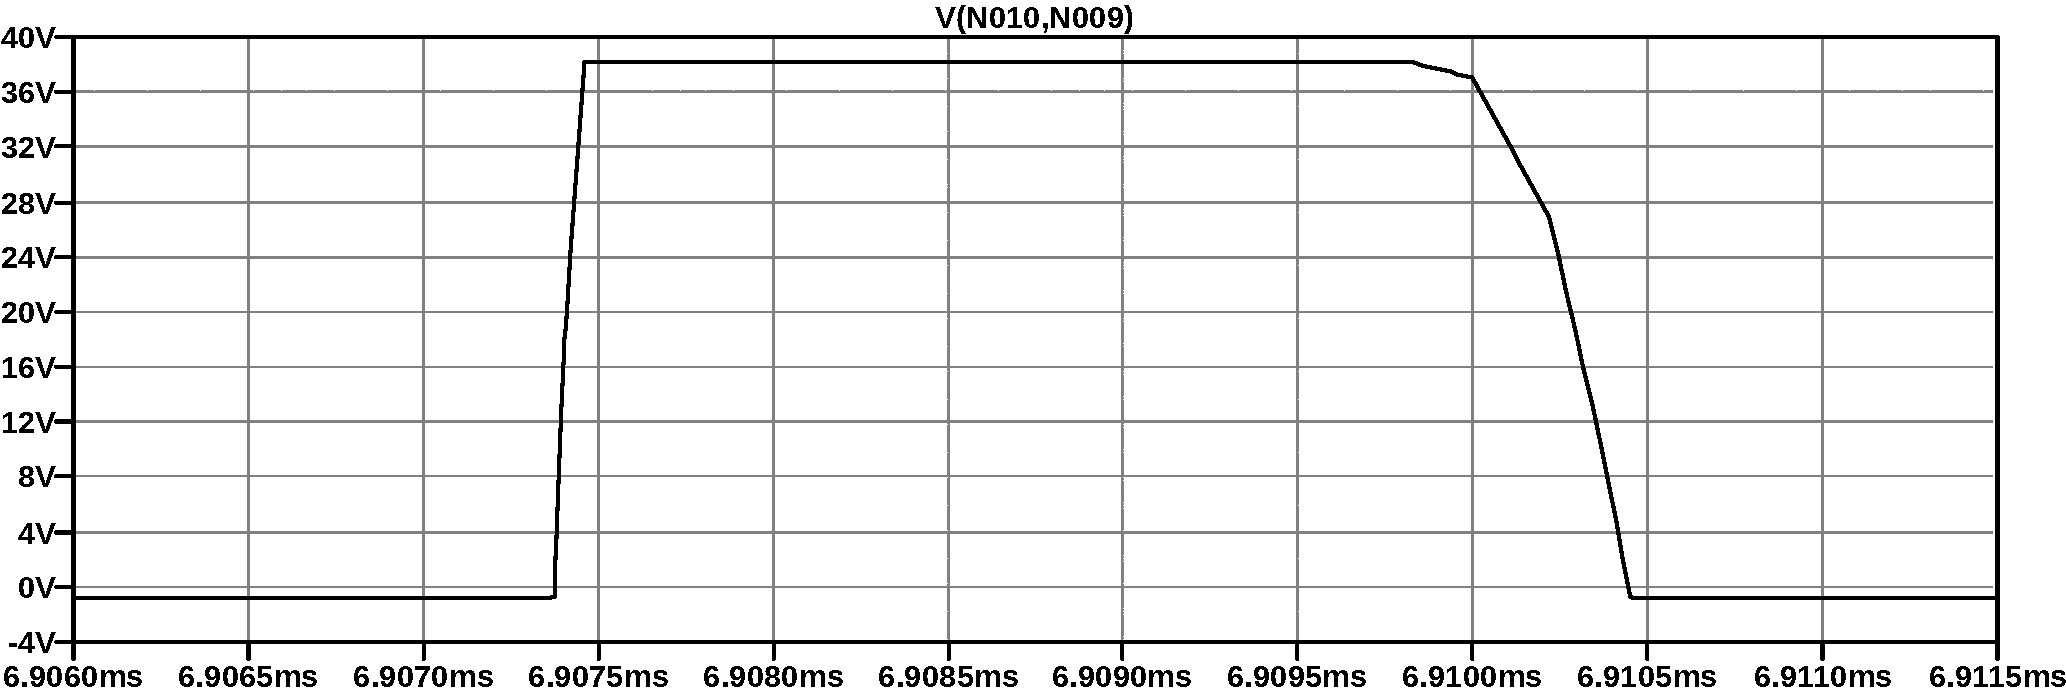
\includegraphics[width=\textwidth]{images/sim/26.pdf}
    \caption{Tensión cátodo ánodo en el diodo D3}
    \label{fig:sim:26}
\end{figure}

\begin{figure}[ht]
    \centering
    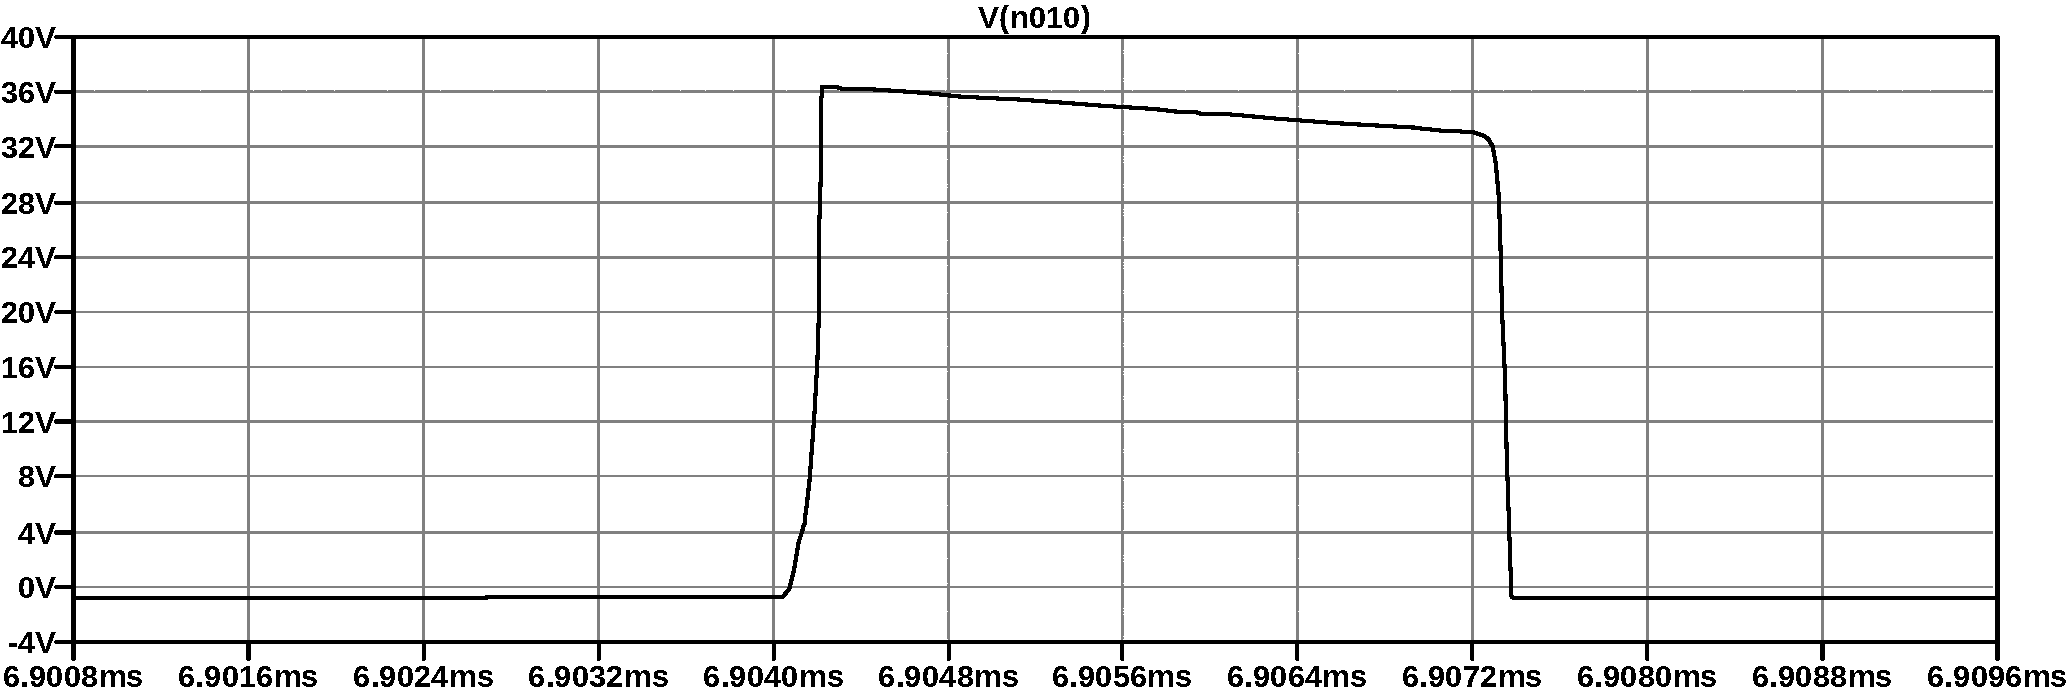
\includegraphics[width=\textwidth]{images/sim/27.pdf}
    \caption{Tensión cátodo ánodo en el diodo D4}
    \label{fig:sim:27}
\end{figure}

\begin{figure}[ht]
    \centering
    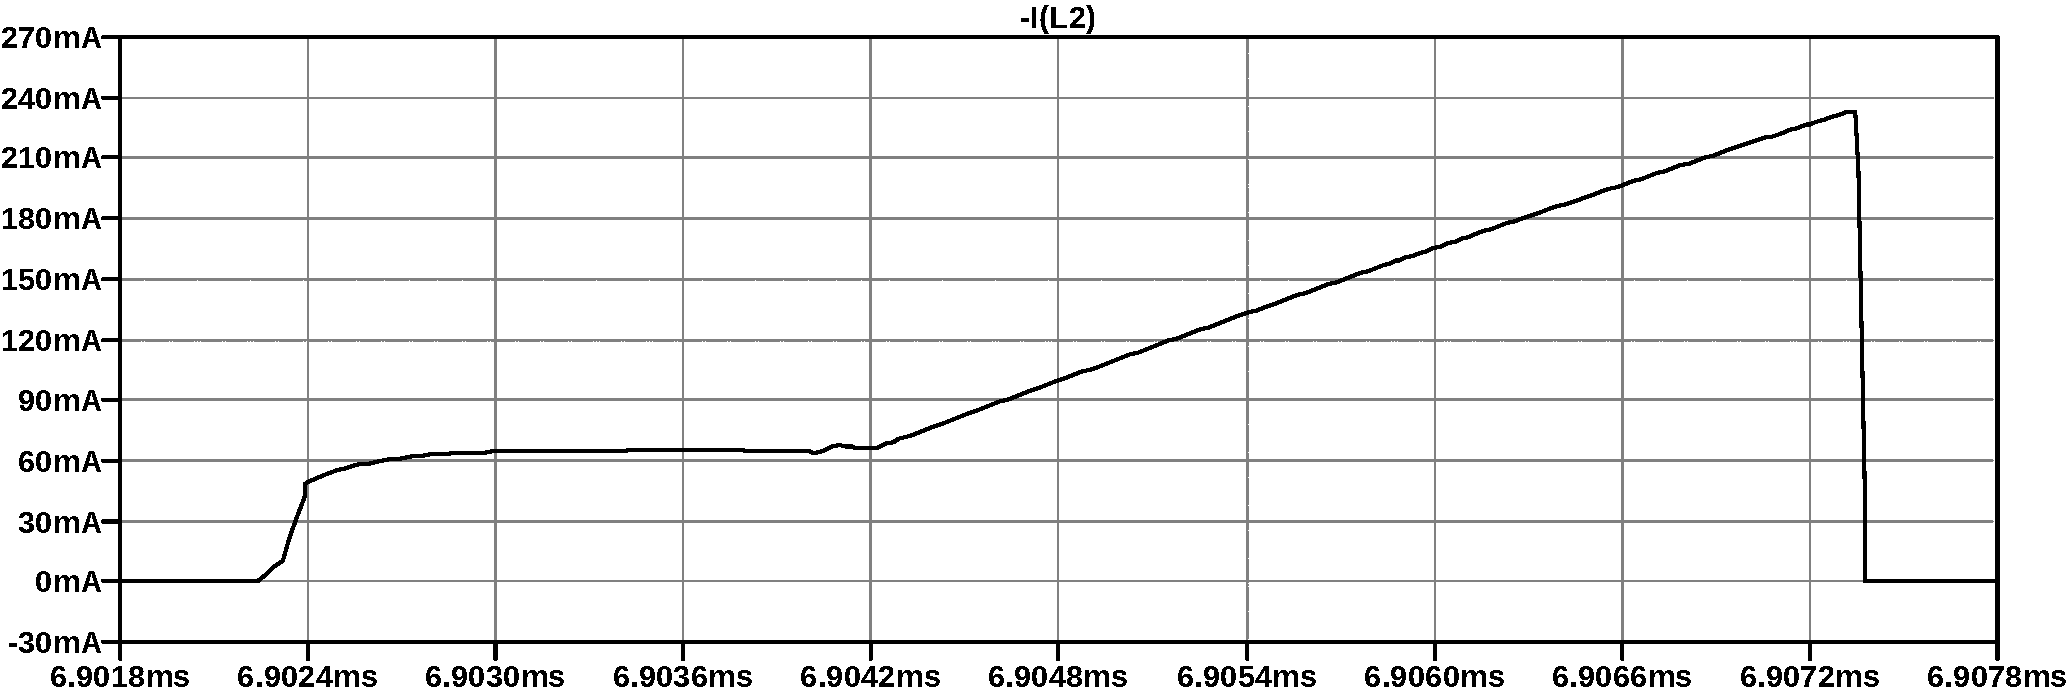
\includegraphics[width=\textwidth]{images/sim/28.pdf}
    \caption{Corriente en el secundario del transformador de potencia}
    \label{fig:sim:28}
\end{figure}
